\documentclass[12pt]{report}
\usepackage{graphicx}
\usepackage{tabularx}
\usepackage{appendix}
\usepackage{pdfpages}
\usepackage[backend=biber, style=authoryear, natbib=true]{biblatex}
\usepackage[colorlinks]{hyperref}
\hypersetup{
colorlinks=false,
pdfborder={0 0 0},
linktoc=all,
linkcolor=black,
citecolor=black,
}
\setcounter{tocdepth}{3}
\addbibresource{references.bib}
\DeclareCiteCommand{\parencite}
  {\ifentrytype{online}{\bibopenparen}{\bibopenbracket}%
   \usebibmacro{prenote}}%
  {\usebibmacro{citeindex}%
   \usebibmacro{cite}}
  {\multicitedelim}
  {\usebibmacro{postnote}%
   \ifentrytype{online}{\bibcloseparen}{\bibclosebracket}}
\graphicspath{{images/}}
\pagenumbering{gobble}
\begin{document}
 \begin{titlepage}
   \begin{center}
        \vspace*{0.5cm}

        \begin{Huge}
        \textbf{Object Detection in Road Images}
        \end{Huge}
        
        \vspace{0.5cm}
        
\includegraphics[width=12cm]{ul} \\
    	
    	\normalsize
        \vspace{1.5cm}
        \textbf{Final Year Project 2019} 
        
        \vspace{0.5cm}
        \textbf{Author: Rory Egan}
        
        \vspace{0.5cm}
        \textbf{ID: 15178668}
 
        \vfill
        \textbf{Bachelor of Science in Computer Systems (LM051)} \\
        \normalsize
        \vspace{0.5cm}
        \textbf{Supervised by}: \textsc{\textbf{J.J. Collins}}
 
  \end{center}
 \end{titlepage}
 
\clearpage
\begin{flushleft}
“DECLARATION
\linebreak
\linebreak
The work described in this document is, except where otherwise stated, entirely that of the author and has not been submitted in any part for a degree at this or any other University.
\linebreak
\linebreak
Signed: \_\_\_\_\_\_\_\_\_\_\_\_\_\_
\linebreak
Dated: \_\_\_\_\_\_\_\_\_\_\_\_\_\_\_”
\end{flushleft}

\begin{abstract}
This project will be a research-oriented project centred around the use of Convolutional Neural Networks (CNN's) for object detection in images from the perspective of a self-driving car. The area of self-driving cars is a rapidly expanding field, with significant investments having taken place over the past several years. Many companies have chosen to use cameras as one of the primary sensors deployed on their prototype cars in conjunction with several other sensors to allow a vehicle to understand its environment and orient itself appropriately. This project will focus on the way these cameras can allow the vehicle to detect different objects in its environment. An important challenge within the field of machine vision in self-driving cars is reliably classifying multiple objects at once within an image. The current standard Machine Learning class of algorithms for object classification are CNN’s. This project will investigate the use of CNN's to analyse colourised 2D images that depict typical scenes presented to a self-driving car and classify the different objects within them. The initial goal is to research and outline the basics of how CNN's operate, then choose a particular CNN paradigm and train an object detector using this paradigm. The CNN should be able to reliably classify major obstacles that are important to the function of a self-driving car such as other vehicles, pedestrians etc. The classifier should aim to be robust to adverse conditions creating variation within the images such as rain, snow etc. This project will also investigate several different types of CNN and document the differences in the ensuing results.
\end{abstract}
\clearpage
\pagenumbering{Roman}
\section*{Acknowledgements}
\begin{flushleft}
First and foremost, I would like to thank my project supervisor, J.J. Collins. I initially came to him in 3rd year with a plan to base my final year project around the subject of Object Detection and Convolutional Neural Networks, and his guidance and knowledge have been instrumental in shaping this project ever since. He has been an exemplary project supervisor, making himself available whenever possible to help.
\linebreak
\linebreak
Secondly, I would like to thank Jamie Mac Manus for the four years of university we have spent together. Without his unwavering discipline and work ethic serving as an example to myself, I can honestly say that my grades would be nowhere near the levels they are at now.
\linebreak
\linebreak
Special thanks are also due to Tom Barrett. His final year project served as the inspiration for this project, and it was him who first set me on the path of investigating self-driving car related datasets.
\linebreak
\linebreak
I would also like to thank Kevin Moynihan and Dan Noonan for all the projects we have worked on together, with them proving to be exemplary teammates.
\linebreak
\linebreak
I have many thanks due to my family and girlfriend, without their continued support and backing I would never have come to the end of my degree. Particular thanks are due to my father for first setting me on the path of Software Development.
\linebreak
\linebreak
Lastly, I would like to thank all of the CSIS staff who have provided guidance and support to me during my time at UL. Without them, none of this would have been possible.
\end{flushleft}
\clearpage
 
\tableofcontents
\listoffigures
\listoftables

\clearpage

\pagenumbering{arabic}
\chapter{Introduction}
\section{Overview of Problem Area}
\begin{flushleft}
Object detection is the process of locating and identifying different types of objects within images (\cite{verschae2015object}), and is a highly researched area in the field of Computer Vision. To gain an understanding of what makes this a difficult task for a computer, one must first understand how images are interpreted by computers. Images are represented as matrices of values, with each value corresponding to a pixel in the image (\cite{learned2011introduction}). Images can be broadly broken down into two groups, grayscale and colour. A grayscale image will be represented as a 2D array of values ranging from 0 to 255, with each value representing the intensity of that pixel, as seen in Figure \ref{fig:pixels}. A value of 0 represents a fully black colour and a value of 255 represents a fully white colour. In grayscale images, each pixel therefore represents one colour channel (gray). In colour images however we have multiple different channels for red, green and blue. In order to represent this, a colour image will be represented as a 3D array of pixel values, with each pixel having 3 values between 0 and 255 associated with it. These three values represent the intensity of the three colour channels at that pixel.
\end{flushleft}

\vspace{0.5cm}
\begin{figure}[ht!]
	\centering
	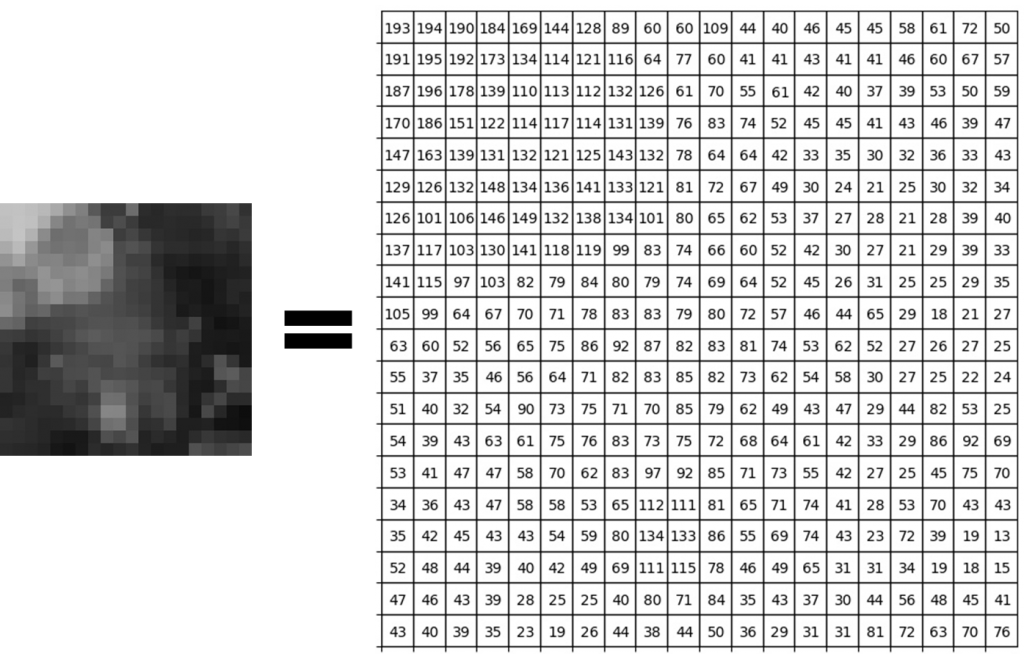
\includegraphics[width=12cm]{pixels}
	\caption{Pixel Representation of Grayscale Image (adapted from https://nrsyed.com/2018/02/17/kernels-in-image-processing/)}
	\label{fig:pixels}
\end{figure}

\clearpage
\begin{flushleft}
The overall goal for object detection algorithms is that they should be able to receive these image representations as input data and return values for the probabilities of different classes existing within the image, as well as provide some information as to where the algorithm predicts that the objects are located, typically in the form of a bounding box (\cite{amit20022d}). This can be seen visualised in Fig \ref{fig:detection}. The overall aim of this project is to train an object detection algorithm that works on a set of images extracted from cameras mounted on cars, containing multiple different objects such as pedestrians, vehicles and traffic lights.
\end{flushleft}

\vspace{0.5cm}
\begin{figure}[ht!]
	\centering
	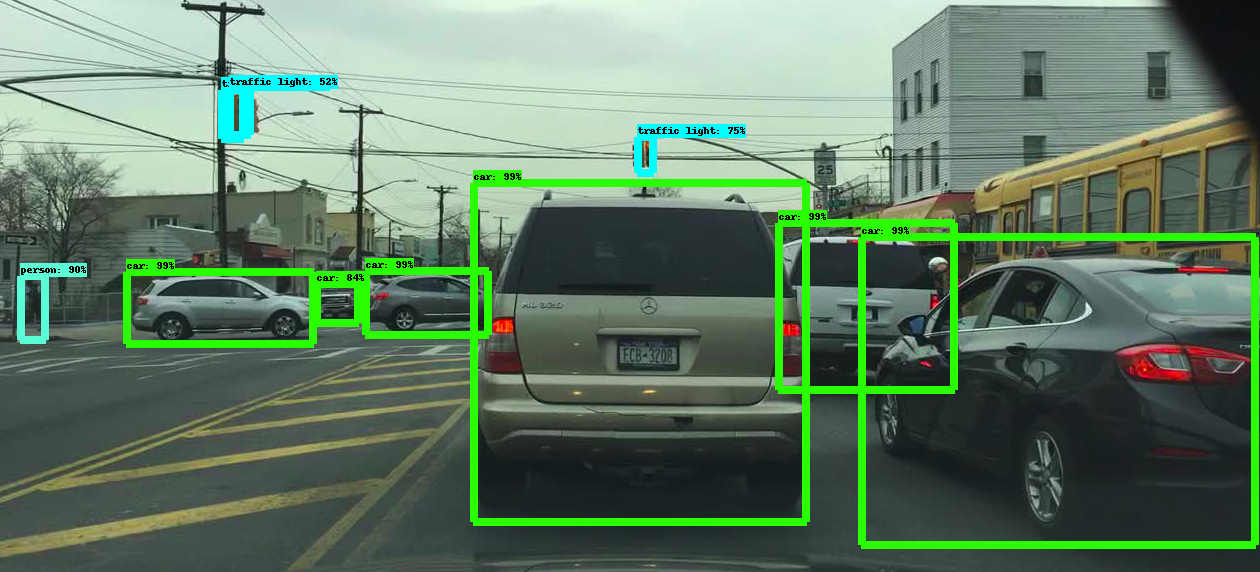
\includegraphics[width=14cm]{detection}
	\caption{Object Detector in action}
	\label{fig:detection}
\end{figure}

\begin{flushleft}
There are many factors that influence the degree to which an object detector is successful. When dealing with images that are extracted from real-life scenarios issues such as illumination and camera focus can cause an image to appear blurry or distorted. As can be seen in Fig \ref{fig:detection} above, objects within images can become partially or fully obscured by other objects. Objects can also change depending on their distance from the camera, further compunding these issues. This means that it can become very difficult to perform object detection to a high degree of certainty upon real-life data (\cite{zhao2019object}). Thankfully, a relatively new form of Machine Learning algorithm known as the Convolutional Neural Network (CNN) has recently risen to prominance that has proven to be quite robust to these complex image-based tasks. This project is based upon the investigation of how CNN's perform upon real-life image data in the context of scenes such as those presented to a self-driving car.
\end{flushleft}

\section{Objectives}
\vspace{0.5cm}
\subsection{Primary Objectives}
\subsubsection*{Utilise a CNN for Object Classification}
The core concept of this project is the use of CNN's for the detection of certain objects present within driving-based images. As such, the primary objective for this project is to research and implement a CNN that will return an acceptable level of accuracy on the testing data. The Berkeley Deep Drive dataset utilised by this project has a related paper in which object detection experiments are run on the dataset and performance metrics from these experiments are recorded (\cite{yu2018bdd100k}). A major objective for this project therefore is to achieve similar results to those achieved in this paper. As an understanding of how CNN's are evaluated is required in order to properly expand upon the results obtained in the paper, the results will be discussed further in a later section.
\subsubsection*{Provide a Visual Interaction With The Trained CNN}
\begin{flushleft}
Once CNN's have been trained to acceptable accuracy levels during the Empirical Studies section, a basic application should be implemented in order for users to observe the CNN in action upon testing data. To this end, a Flask application is to be developed that will allow users to upload images upon which object detection will take place. As the Berkeley Deep Drive dataset contains videos as well as images, object detection should take place on a small number of test videos in order to provide users an example of how a CNN operates in real-time.
\end{flushleft}
\subsection{Secondary Objectives}
\subsubsection*{Understanding of CNN's}
As this is a primarily research based project, one of the main objectives is to gain a deep understanding of how CNN's operate. The following sections of this report should demonstrate a depth of knowledge around the theory of how CNN's work, as well as demonstrate an ability to put these theories into practice. The section on Empirical Studies in particular should demonstrate an ability to forensically examine the results produced from CNN's and provide insight into how these results are achieved.
\vspace{0.5cm}

\section{Contribution}
\begin{flushleft}
Although results of applying a CNN to the Berkeley Deep Drive dataset have been published in (\cite{yu2018bdd100k}), the authors of this study only used one particular architecture of CNN to obtain their results. This report outlines results obtained using two different types of CNN architecture across a range of different types of experiment. As the Berkeley Deep Drive dataset is a newly released dataset from 2018, a large body of research has yet  to be carried out on the dataset. As such, this report may be of some small use to aid in avoiding some of the problems encountered during this project.
\end{flushleft}

\section{Methodologies}
\begin{flushleft}
\begin{enumerate}
\item Define the Research Area: The first step in this project was to define which problem domain to base this FYP around. As an avid SCUBA diver, the initial area I investigated was the field of fish classification in images and videos collected from Irish waters. This area appealed to me as I wanted to investigate the possibility of collecting the dataset myself using underwater camera equipment. However I quickly abandoned this area for several reasons:
\begin{enumerate}
\item Equipment: Underwater camera equipment that is capable of taking high resolution images and videos is extremely expensive. Due to the strenuous nature of diving in rough Irish waters, equipment with excellent stabilisation software would be required in order to reliably obtain non-blurred images.
\item Domain Knowledge: As I am not an expert in the field of fish identification, I would be unable to reliably annotate species present in the training images. This would require enlisting the help of a third-party expert in the field of fish species.
\item Time Constraints: There are no datasets currently available that contain annotated fish species in underwater images or videos in Northern Atlantic waters. As such, the full dataset would need to be collated and annotated myself. With time constraints present for this project, it would not be feasible to carry out all this work in time to reach project deadlines.
\end{enumerate}
With these issues present for my initial choice of problem domain, I decided to instead focus on the area of road images as there have been several large-scale annotated datasets released in recent years that I could leverage. Moreover, after receiving a graduate offer from Jaguar Land Rover I decided that this project could serve as an excellent introduction into the problems faced by automotive companies in the field of Computer Vision.
\item Background Research: The next step was to carry out a literature review around the topic of Neural Computing, specifically CNN's. Papers dealing specifically with the challenges presented during object detection were the main focus of the literature review. In an attempt to demonstrate an understanding of how CNN's operate, the literature review has been summarised in the following sections of this report.
\item Gain a hands-on knowledge of tensorflow: As tensorflow was the tool utilised to implement CNN's during this project, a Udemy tutorial was first followed in an attempt to gain an understanding of using tensorflow in a hands-on manner (\cite{udemy}).
\item Carry out Empirical Studies: Empirical Studies were a major point of focus for this project. Experimentation was carried out on the Berkeley Deep Drive dataset using a range of different types of CNN. Results from these experiments were documented and investigated in order to gain an understanding of what techniques work best for the dataset. The results from the experiments were then compared to results carried out in (\cite{yu2018bdd100k}).
\item Build an application: Once Empirical Studies had been carried out and CNN's had been trained on the Berkeley Deep Drive dataset to a satisfactory degree, a prototype application was built to allow users to observe the Object Detection taking place.
\end{enumerate}
\end{flushleft}

\section{Motivations}
\begin{flushleft}
The main motivation behind this project for me is working within the field of self-driving cars. I have previously worked a summer internship at Jaguar Land Rover in Shannon working within the ADAS (driver assistance) team. I was exposed to a broad range of different technologies, from Computer Vision and Machine Learning based teams to Big Data pipelines concerned with offboarding data from test cars. This internship and the receipt of an offer to return to the company as a graduate has motivated me to further my study within this field. I have found that these technologies are much more interesting to me than many more conventional potential areas of work. With ever increasing amounts of automotive manufacturers investigating this field, I feel like a final year project focusing on self-driving cars could be very beneficial to my career going forward.

I am also very interested in self-driving cars due to the far-reaching safety implications of the technology. Hundreds of people die on Irish roads every year, with driver error being the primary cause of fatalities. Driver distraction has been reported as the cause of one in seven accidents that take place in Ireland (\cite{rsadistraction}). Self-driving cars have the potential to significantly increase road safety once fully autonomous capability has been reached (\cite{milakis2017policy}), and I find it very motivating to work within a field that genuinely has the potential to save lives. Outside of the direct safety implications of self-driving cars, they have also shown the potential to have positive environmental effects through a reduction of fuel wastage (\cite{greenblatt2015autonomous}). I believe that this technology is certainly a field in which I can leave a positive and lasting impression on the world.
\end{flushleft}

\chapter{Background Research}
\section{Autonomous Vehicles Overview}
\begin{flushleft}
Before the areas of Machine Learning and CNN's are discussed, it is important to first put into context why these areas matter to an autonomous vehicle. Although driver assistance features such as lane assist, parking assist etc. are prevalent in much of the luxury car market today, a truly self-driving car has yet to be brought to market. A truly self-driving car is a wheeled, autonomous robot that is capable of traveling between destinations without human intervention based on information received from automotive sensors, regardless of road or weather conditions (\cite{zhao2018key}). Autonomous vehicles are discussed in the context of levels of autonomy, with each level representing a step closer to fully autonomous capabilities. The most widely accepted definition for the differing levels of autonomy was published by SAE international, with six distinct levels being distinguised by the level of driver attentiveness and involvement required (\cite{sae2016taxonomy}). This publication breaks down the levels of autonomy as follows:

\begin{itemize}
\item Level 0: System may issue warnings, however no sustained vehicle control is present.
\item Level 1: Control of the vehicle is shared between the driver and the system - for example adaptive cruise control.
\item Level 2: System is capable of taking full control of the vehicle under certain conditions such as highway driving, however the driver must be prepared to intervene at any moment.
\item Level 3: Driver is capable of taking their attention away from driving, however they must be capable of intervening when the system alerts.
\item Level 4: Similar to level 3, however less driver attention is required. Inside of specific "geofenced" areas and favourable weather conditions, the vehicle is capable of driving in an autonomous manner. However, the vehicle must be able to abort the trip if driver does not take control when the system alerts them - ie. park the car at the side of the road.
\item Level 5: Full autonomy, no human intervention required at any point during the trip.
\end{itemize}
\end{flushleft}

\vspace{0.5cm}
\begin{flushleft}
The technologies present within a self-driving car can be split into four distinct categories - environment perception, car navigation, path planning, and car control (\cite{zhao2018key}). The technologies focused on in this project relate to the perception module, which handles how the vehicle perceives its surrounding environment, allowing the vehicle to make informed control and planning decisions. The perception module generally consists of several different types of sensors with the main types consisting of radar, LIDAR and camera systems. These sensors operate as follows:
\begin{itemize}
\item Camera: Standard camera units, typically producing 30 or 60 frames per second.
\item Radar: Standing for Radio Detection and Ranging, it works by generating high-frequency radio waves which bounce back off objects and are then processed. The Doppler effect allows radar units to measure the speed of objects, allowing a self-driving car to calculate the relative velocities of other vehicles (\cite{kocic2018sensors}).
\item LIDAR: Standing for Light Detection and Ranging, LIDAR is a relatively new form of sensor. Operates in a broadly similar manner to a radar unit, however it uses an infrared laser beam in the place of radio waves. Most LIDAR units consist of a swivelling device, allowing them to create a 3D map of objects around the vehicle.
\end{itemize}

\vspace{0.5cm}
Although each of these sensors has their own distinct advantages and disadvantages, this project focuses on the information created by camera sensors. The reason for this is due to the fact that cameras are widely accepted as a major part of any autonomous car system currently being developed (\cite{kocic2018sensors}). The reasons for camera sensors being so prevalent within the industry are as follows:
\begin{itemize}
\item Cost: Cameras are among the least expensive sensors available to automotive manufacturers. A major concern with other sensors such as LIDAR is the availability of sensors that are cheap enough to feasibly be mounted on production cars.
\item Colour: Cameras are capable of returning colour information, which is an important part of many detection tasks.
\item Power: Cameras typically require very little power input in order to run.
\end{itemize}

\vspace{0.5cm}
Their cost effectiveness and colourised output ensure that cameras are likely to remain an integral part of autonomous vehicle systems for years to come. Due to the immaturity and cost of LIDAR technologies, Tesla have controversially decided to eschew LIDAR sensors altogether in favour of camera, radar and ultrasonic sensors, with certain arguments being put forth that cameras will replace LIDAR entirely in the future (\cite{harris2015cheaper}). Regardless of which particular configuration of sensors are utilised in different autonomous vehicle solutions, cameras remain the main sensor utilised by most manufacturers (\cite{kocic2018sensors}). As such, it was decided that this project would focus on image data that has been generated from cameras.
\end{flushleft}

\vspace{0.5cm}
\begin{flushleft}
Once data has been generated by a sensor, it must be acted upon in some way by the autonomous system. The different ways in which the system will act upon the received data is determined through the "learned" experience available to the system in the form of some type of Machine Learning algorithm (\cite{surden2016technological}). The standard type of Machine Learning algorithm that is utilised for image based problems is the Neural Network, a class of Machine Learning algorithm modelled off the neural pathways of the brain. Within this class of algorithm, a CNN's have become increasingly popular due to their suitability for tackling image based problems. Both Neural Networks and CNN's will be explained further in this paper, however it should now be apparent what role a CNN performs within the overall architecture of an autonomous vehicle.
\end{flushleft}

\section{Introduction to Machine Learning}
\begin{flushleft}
A general definition of Machine Learning:
``[Machine Learning is the] field of study that gives computers the ability to learn without being explicitly programmed`` - Arthur Samuel, 1959.

One of the goals for Machine Learning algorithms is automatically observing structures in data and fitting these structures to a model in order to allow people to interact with the data in a way that is humanly intuitive.

Development within the field has progressed to the point where people interact with Machine Learning algorithms multiple times in their daily lives without noticing. Areas such as email spam detection, Facebook image tagging suggestions and voice-to-text are all examples of a broad range of Machine Learning algorithms that are commonly used.

Machine Learning can be roughly divided into two categories - Supervised and Unsupervised. 
\end{flushleft}

\subsection{Supervised Learning}
\begin{flushleft}
In Supervised Learning, algorithms are provided with some labelled input data which they attempt to learn patterns from. The algorithms will then attempt apply this learned experience to new unseen data and attempt to create their own labels for the data, with varying degrees of success. Prominent examples of the Supervised category of Machine Learning include Support Vector Machines, Linear Regression and the focus of this project, Convolutional Neural Networks (\cite{o2015introduction}).
\end{flushleft}

\subsection{Unsupervised Learning}
\begin{flushleft}
Unsupervised Learning algorithms differ from Supervised Learning algorithms in that they are given data with no labels. They must then attempt to find some structure in this input data themselves with no given direction or explicit programming. Popular Unsupervised Learning examples include clustering algorithms.
\end{flushleft}

\subsection{History of Neural Computing}
\begin{flushleft}
Neural Networks are not a new concept - they were first proposed in 1943 by neurophysicists in the form of a primitive electrical circuit. The concept was studied up until the 1960's until it fell out of favour with researchers. Bold claims had been made by many researchers about the vast potential of the field, however a failure to back up these claims led to widespread skepticism about the true potential of Neural Computing. The area was in part hampered by the technology of the time - processing power available to researchers was very low. Additionally, in 1969 a paper was published introducing the XOR problem, which will be explained in later section. The paper stated that the research being carried out at the time on Neural Networks was fundamentally flawed and that the field would not experience any major successes (\cite{minsky1969introduction}). A revival was seen in the 1980's, when the concept of using multiple layers of neurons to create a network began to emerge, and the issues presented by the XOR problem were solved. From 1989 to 1994 Yann LeCun developed the LeNet architecture, one of the first examples of a CNN, which was used to recognise handwritten postal addresses. In around the 2010 the field of Deep Learning (explained below) experienced a surge in popularity, primarily due to the increase in processing power made available through GPU's. In 2012, Alex Krizevsky won the ImageNet competition, a popular image recognition competition. The architecture he used, known as AlexNet, achieved an error rate of ~15\%, which was approximately 10\% better than the closest competition at the time. His architecture essentially scaled up the LeNet architecture into a larger, more complex network (\cite{krizhevsky2012imagenet}). This architecture caused a widespread adoption of CNN's within image based Machine Learning, and CNN's are now the de facto standard for many image processing tasks (\cite{o2015introduction}).
\end{flushleft}

\section{Introduction to Neural Networks and Deep Learning}

\begin{flushleft}
Artificial Neural Networks (ANN's) are a particular Supervised Machine Learning paradigm modelled after the neural pathways present in the brain. The building blocks for every Neural Network are called perceptrons or nodes, and can be thought of as artificial neurons. A perceptron receives inputs with weights associated with them that show the importance of each input relative to the others. The perceptron applies a particular activation function with a bias attached to the weighted sums of the input, and an output is generated, as shown in Figure \ref{fig:neuron} (\cite{geron2017hands}).
\end{flushleft}

\vspace{0.5cm}
\begin{figure}[ht!]
	\centering
	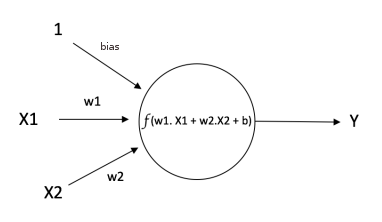
\includegraphics[width=10cm]{neuron}
	\caption{An Artificial Neuron (adapted from https://ujjwalkarn.me/2016/08/09/quick-intro-neural-networks/)}
	\label{fig:neuron}
\end{figure}

\begin{flushleft}
A single Perceptron is only able to classify linearly separable data (\cite{kotsiantis2007supervised}). In order to classify data that is not linearly separable, techniques such as Multilayer Perceptrons must be used. These will be explained in a following section. Linear separability refers to the ability for a single line to separate all members of a given class A from all members of a given class B. This is illustrated in Figure \ref{fig:linear}.
\end{flushleft}

\vspace{0.5cm}
\begin{figure}[ht!]
	\centering
	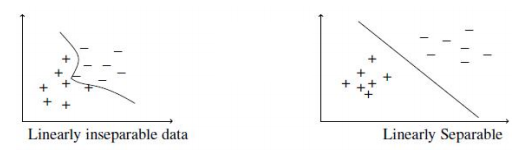
\includegraphics[width=10cm]{seperable}
	\caption{Linearly Separable vs Inseperable (adapted from \cite{mohamed2017comparative})}
	\label{fig:linear}
\end{figure}

\begin{flushleft}
There are several different types of activation function, however every activation function takes in a single number as input and performs a certain mathematical operation on the number. The three most common activation functions generally encountered are ReLU, tanh and sigmoid. Rectified Linear Unit, or ReLU, takes in an input and replaces negative numbers with zero. The tanh function squashes the input to between the range between -1 and 1. Finally the sigmoid activation function takes the input and squashes it to the range between 0 and 1. In the field of CNN's ReLU is commonly used, as training times are significantly better when using this activation function. (\cite{krizhevsky2012imagenet}). These different types of activation function are visualised in Figure \ref{fig:functions}.
\end{flushleft}

\vspace{0.5cm}
\begin{figure}[ht!]
	\centering
	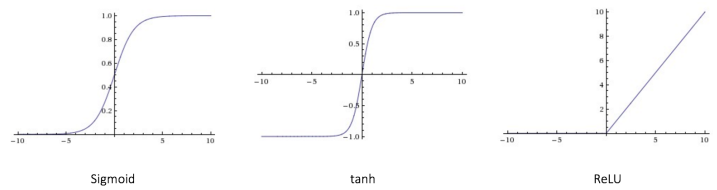
\includegraphics[width=12cm]{functions}
	\caption{Activation Functions Visualised (adapted from https://towardsdatascience.com/activation-functions-in-neural-networks-58115cda9c96}
	\label{fig:functions}
\end{figure}

\begin{flushleft}
A Neural Network consists of a series of interconnected layers of these artificial neurons, with the output of each layer of neurons serving as input for the next layer of neurons. The simplest and most common type of Neural Network is the feedforward neural network. It consists of multiple layers of neurons, with connections to all of the neurons in the preceding layer. Each connection or edge has a weight associated with it. There are three types of nodes - input nodes, hidden nodes and output nodes. As the name suggests, data in a feedforward neural network only moves forward through the network - into the input layer, through the hidden layers and then on to the output layer.
\end{flushleft}

\subsection{Input Nodes}
\begin{flushleft}
Input nodes take in the input data fed into the network without performing any computation and pass the data on to the hidden nodes. These nodes make up the input layer of a neural network.
\end{flushleft}

\subsection{Hidden Nodes}
\begin{flushleft}
The hidden nodes perform the actual computation, taking data from the input nodes and providing information to the output nodes. There can be multiple or zero hidden layers in a network, whereas there will only ever be one input and output layer.
\end{flushleft}

\subsection{Output Nodes}
\begin{flushleft}
Like the input nodes, the output nodes do not perform any computation on the data - they simple take information from the hidden layers and expose this to the outside. This will generally consist of a prediction.
\end{flushleft}

\subsection{XOR Problem}
\begin{flushleft}
In the paper mentioned above, "Perceptrons: An Introduction to Computational Geometry", the Xor problem was first introduced. Xor is a function that given two binary inputs returns 0 if the inputs are equal and 1 if they are not. Xor is a classification problem with known expected results, therefore it is appropriate to utilise a Supervised Learning approach to solving it. However, the Xor problem is an example of a problem that is not linearly seperable. As mentioned previously, a single perceptron is not capable of predicting data that is not linearly seperable, therefore a single layered architecture of perceptrons is simply not capable of solving this problem. The only way for a Neural Network to solve this problem is to expand the number of layers in the architecture, adding a hidden layer. This type of architecture is known as the Multilayer Perceptron.
\end{flushleft}

\subsection{Multilayer Perceptron}
\begin{flushleft}
A Multilayer Perceptron (MLP) consists of an input layer, an output layer and one or more hidden layers, as seen in \ref{fig:mlp}. MLP's are feedforward neural networks, with the output of each node in the network serving as the input for every single node in the next layer. This concept of having each node taking inputs from every single node in the preceding layer is referred to as "fully-connected" layers. "Deep Learning" is when there is more than one hidden layer present in a network (\cite{o2015introduction}). 
\linebreak
\linebreak
The MLP architecture solves the Xor problem by introducing linear seperability (\cite{Singh2016MinimumCM}) through the addition of these extra layers of perceptrons. The purpose of the extra layers is to provide an input for the next perceptrons in the next layer in the network until the output layer - resulting in a linearly seperable problem.
\linebreak
\linebreak
Learning takes place in a MLP through changing the connection weights for each perceptron in the network based on the error between the expected and true output of each perceptron. This is carried out through a concept known as backpropagation.
\end{flushleft}

\vspace{0.5cm}
\begin{figure}[ht!]
	\centering
	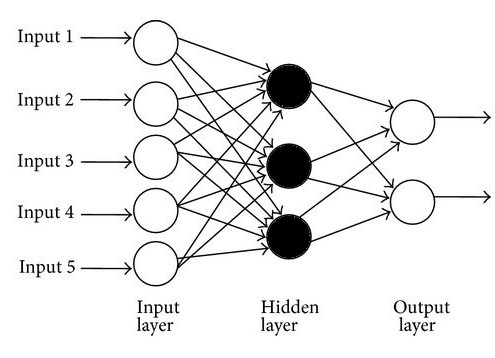
\includegraphics[width=12cm]{mlp}
	\caption{Multilayer Perceptron Architecture (source: https://medium.com/pankajmathur/a-simple-multilayer-perceptron-with-tensorflow-3effe7bf3466)}
	\label{fig:mlp}
\end{figure}

\newpage
\subsection{Gradient Descent and Backpropagation}
\begin{flushleft}
Gradient descent is an algorithm used to optimise the weights between neurons in such a manner that creates the least possible amount of error. When the network is training, a cost function is used to keep track of how the network is performing. The cost function looks at the discrepancies between the training output and the true values to determine an error. When the network trains, the goal is to therefore get this cost function as low as possible to ensure the lowest possible error (\cite{rumelhart1985learning}). The way the cost function is minimised in an MLP is through gradient descent and backpropagation.

Every time the weights must be updated, the derivative of the cost function with regards to the weight itself scaled to a learning rate is subtracted. As the network trains the derivative should decrease with each training iteration. This is known as gradient descent. When the cost function cannot be reduced any more, it has converged.

The backpropagation algorithm works in conjunction with this by starting at the output layer of the network and stepping back through all the layers, updating the weights for each neuron as it goes (\cite{rumelhart1985learning}). This is in an attempt to minimise the overall error. These steps should allow the network to reduce its error and converge on an optimal solution over time as the network trains.
\end{flushleft}

\section{Computer Vision}
\subsection{Noise and Occlusion}
\begin{flushleft}
Within any image dataset that contains images extracted from real-life scenarios, two commonly used terms are noise and occlusion. Image noise is the presence of random variation in pixel colour and intensity within images, typically produced by the sensor taking the image. Within the Berkeley Deep Drive dataset, a common source of noise is motion blur produced by the camera taking a picture while the test car is in motion. This type of image noise can be observed in Fig \ref{fig:noiseimg}. A proliferance of noisy images within a dataset should be avoided if possible, as an overly noisy dataset will cause classifier performance to suffer (\cite{xiao2015learning}).
\end{flushleft}

\vspace{0.5cm}
\begin{figure}[ht!]
	\centering
	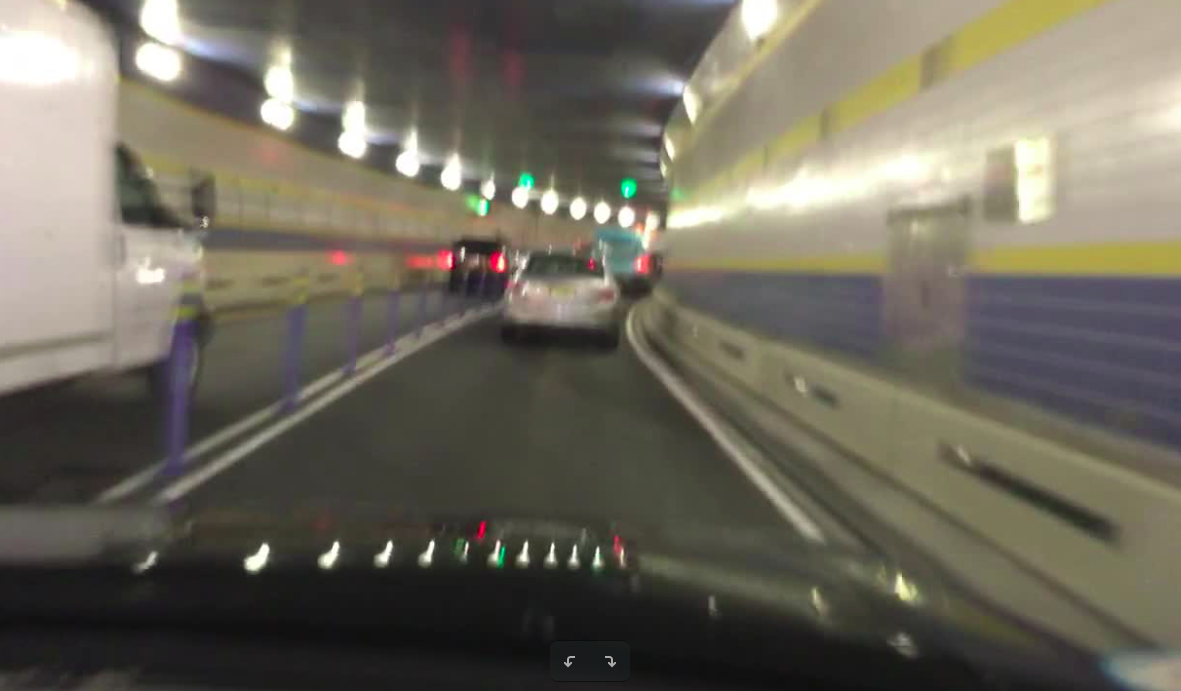
\includegraphics[width=12cm]{noise}
	\caption{Image noise produced by motion blur}
	\label{fig:noiseimg}
\end{figure}

\newpage
\begin{flushleft}
Occlusions within an image are when a particular object is covered in some way, making it only partially visible. This is problematic for classification as it hides some features of the object, making it more difficult for the classify to determine what class the object belongs to. In the Berkeley Deep Drive dataset this is typically present in long rows of cars occluding each other as seen in Fig \ref{fig:occlusion}.
\end{flushleft}

\vspace{0.5cm}
\begin{figure}[ht!]
	\centering
	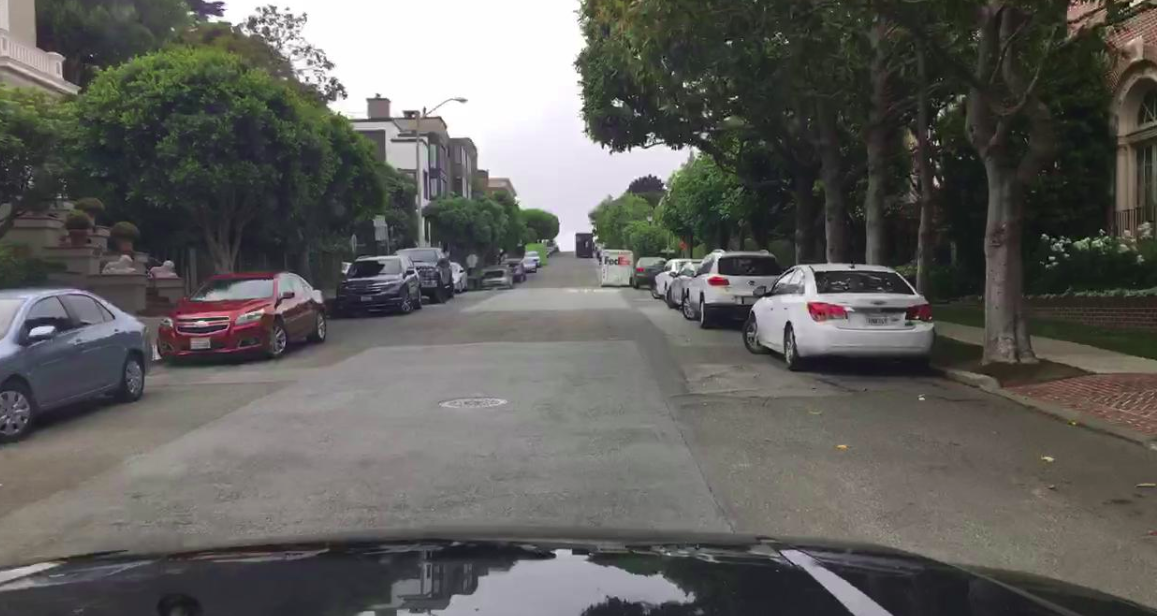
\includegraphics[width=12cm]{occlusion}
	\caption{Image containing occluded cars}
	\label{fig:occlusion}
\end{figure}

\newpage
\subsection{Edge Detection}
\begin{flushleft}
Edge detection is the ability to recognise object boundaries within an image, with most edge detection techniques using changes in pixel intensities to identify potential edges (\cite{arbelaez2011contour}). Although edge detection may appear straightforward in concept, in practice it can be a difficult task. Input images typically suffer from noise due to focal blur, as well as blur caused by shadows. This can cause smoothing in the variations in pixel intensity at edge points, and make it difficult to define what actually is an edge (\cite{ziou1998edge}). The magnitude of a gradient will determine if a point in the image is an edge or not - a high gradient implies that an edge is likely present. The direction of a gradient shows how the edge is oriented within the image.
\end{flushleft}

\subsubsection*{Approaches}
\begin{flushleft}
There are a multitude of different techniques used for edge detection that can be split into two categories, search based and zero-crossing based. Search based techniques work by computing gradient edge strength, then searching for the direction of the edge by computing the gradient orientation. The Sobel operator is an example of this type of technique (\cite{gupta2013sobel}). Zero-crossing based techniques differ in that they search for zero-crossing points on a second-order derivative function calculated from the image. Generally smoothing is applied to the image prior to any of these technques (\cite{ziou1998edge}).
\end{flushleft}

\subsection{Multilayer Perceptron for Image Tasks}
\begin{flushleft}
Prior to the popularisation of the CNN, MLP's were the standard for image based problems. However, there are several issues that make the MLP quite unsuitable for this type of problem.

\vspace{0.5cm}
The main issue with MLP's is the manner in which they receive input data. As mentioned above, pixel representations of colour images consist of 3D arrays of pixel values. In order for this data to be passed into an MLP, it must be "flattened" into a 2D vector - as each input node in the MLP accepts a single pixel value (\cite{ben1999fast}). This disregards the spatial characteristics of the image, as the image has been transformed into a large vector of pixel values. This is a very inefficient way of processing images, as it stands to reason that the spatial relationships between pixels are important ie. if two pixels are close together it is likely that they are related in some way (\cite{lecun1989backpropagation}). This lack of consideration for spatial relationships means that an MLP must be given training data that consists of labelled classes in a range of different positions and levels of occlusion within the training images in order for it to reliably identify the classes when it is applied to unseen data, rather than being able to identify a class regardless of its position within an image. Although an MLP may perform adequately upon very simple target domains, more complex tasks will require a large amount of training data in order to produce a reliable classifier (\cite{ghaith}).

\vspace{0.5cm}
MLP's also encounter other issues when attempting to carry out classification tasks on large input images. As mentioned, each pixel of an input image must correspond to an input node in the network. As every node is connected to every other node in its preceding layer, large images quickly require a large amount of nodes in the network. A small image of size 28x28 pixels such as the images found in the MNIST dataset will require a network with 784 input nodes. Images sourced from the Berkeley Deep Drive dataset are of size 1280x720 pixels, which would require an input layer consisting of 928080 nodes. This means that an MLP that takes in large input images requires a huge number of parameters. Computing all of these parameters naturally leads to extremely long training times.

\vspace{0.5cm}
So, it should now be clear that the manner in which MLP's handle image related tasks could be much more efficient. It is with these issues in mind that CNN's were developed (\cite{lecun1989backpropagation}).
\end{flushleft}


\section{Introduction to Convolutional Neural Networks}
\begin{flushleft}
When humans look at an image of say, a dog, we automatically extract the things we have learned that make a dog unique in order to allow us to recognise it. For example we may see a tail, fur and a snout and recognise that we are looking at a dog. At an extremely high level this what a CNN will do - it will look for certain low-level aspects of the object known as "features" such as curves and edges, building these up into more abstract concepts such as a leg or a tail in order to determine what features the object is comprised of, thus allowing it classify the object (\cite{lecun1995convolutional}).
\end{flushleft}

\begin{flushleft}
Interestingly enough, CNN's do take some inspiration from how the brain processes images. The visual cortex of the brain contains many fields that are sensitive to different specific elements of the input. Some groups of neurons will only respond when certain elements of the input are present, for example certain vertical edges, and other groups of neurons will respond to different elements, such as horizontal edges (\cite{youtube}). The concept of distinct groups of neurons looking for certain features is one that has translated very well into Computer Vision through the use of CNN's. The most important aspect of CNN's that improve their suitability for image related problems is the manner in which they detect classes regardless of their position within an image (\cite{albawi2017understanding}) ie. a CNN trained to detect faces does not pay any regard to where instances of faces are located within an image, it simply recognises them. The main point of note when trying to understand what distinguises CNN's from traditional Machine Learning approaches is that they preserve the matrices that the images are represented as, preserving the relationships between pixels rather than simply unpacking the images into long vectors (\cite{lecun1995convolutional}). Instead, they observe groups of pixel values within the matrices in order to process the data contained within them. They do this through special types of layers known as Convolution and Pooling layers.
\end{flushleft}

\subsection{Convolution Layer}
\begin{flushleft}
There are three important points of note regarding the Convolution layer. These are the input image, the feature detector and the feature map. The input image is the image which the CNN is given. The feature detector is a matrix (usually 3x3 or 7x7), also called the kernel or filter, which is multiplied against matrix values of regions within the input image to create what is known as a feature map, with the aim of capturing only important features of the input image. The way this works is the feature detector slides or "convolves" over the whole image (\cite{o2015introduction}). The particular point on the image that the feature detector is analysing is known as the receptive field. 
\linebreak
\linebreak
The parameter known as the stride is the value of the number of pixels by which the feature detector convolves over the input image. For example, a stride of 2 will convolve the feature detector over the input image jumping 2 pixels at a time. As the feature detector convolves around the input image, the pixel values of the feature detector are multiplied against the pixel values of the receptive field. These multiplications are all summed to give a single value. The higher the value, the higher the likelihood that the particular feature represented in the feature detector is present in the receptive field. The feature detector then continues to carry out this process for every section of the input image. The output of this process is a range of new 2D arrays of potentially important features of the input image known as feature maps (\cite{zhao2019object}), as shown in Figure \ref{fig:conv}. As multiple filters are applied at each layers, images are "deepened" ie. an image that is 32x32x32 (a 32x32 image with 3 colour channels) that has 9 filters applied will result in a matrix of dimensions 32x32x9. Each of these 9 layers represents the original image, however they now contain feature information rather than colour values (\cite{lecun1995convolutional}).
\linebreak
\linebreak
A benefit of this process is that the layers of a CNN do not need to be fully-connected as in an MLP, rather they need only be connected to neurons close to them in a principle known as local connectivity - the input of a neuron is received from a small local group of pixels (\cite{lecun1995convolutional}). Local connectivity is made possible due to the fact that the CNN does not alter the structure of the image as in an MLP, instead related pixels remain close together. Due to the fact that neurons are only connected to a small number of other neurons, the number of parameters required to be computed by the network is reduced, and therefore the overall computation time is reduced.
\end{flushleft}

\vspace{0.5cm}
\begin{figure}[ht!]
	\centering
	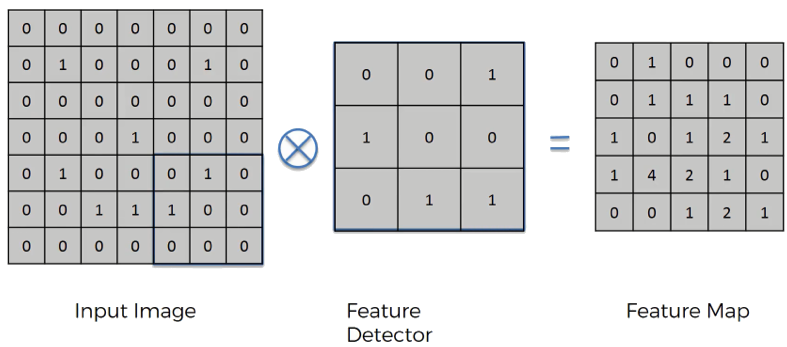
\includegraphics[width=12cm]{conv}
	\caption{Convolution taking place (source: https://www.superdatascience.com/blogs/convolutional-neural-networks-cnn-step-1-convolution-operation/)}
	\label{fig:conv}
\end{figure}

\newpage
\subsection{Pooling Layer}
\begin{flushleft}
The pooling layer performs downsampling to extract key important features and reducing the number of parameters in the network. The pooling layer operates over every feature map by placing a matrix over the feature map and selecting the min value, max value or mean value, depending on the type of pooling being utilised, as shown in Figure \ref{fig:pool}. These extracted values form the pooled feature map (\cite{o2015introduction}). Thus, pooling layers serve to reduce the width and height of an image while preserving only the most important features that have been extracted by the filters in the convolution layer (\cite{zhao2019object}).
\end{flushleft}

\vspace{0.5cm}
\begin{figure}[ht!]
	\centering
	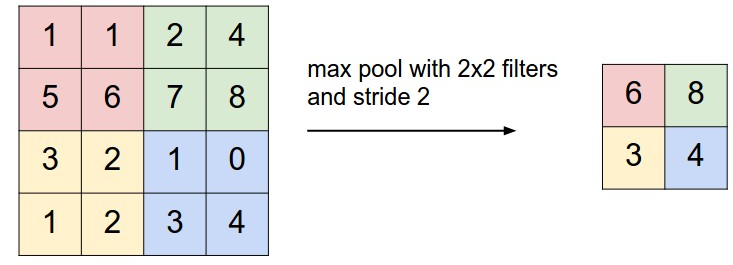
\includegraphics[width=12cm]{pool}
	\caption{Pooling (adapted from: http://www.peculiar-coding-endeavours.com/2018/mlp\_vs\_cnn/)}
	\label{fig:pool}
\end{figure}

\begin{flushleft}
The architecture of a CNN follows essentially the same architecture as a standard MLP, with the addition of these extra layers of Convolution and Pooling. When these layers of Convolution and Pooling are stacked with a fully-connected layer, a CNN architecture has been formed. Once all of the Convolution and Pooling steps have been performed, a fully-connected layer will compute the overall class scores, resulting in a final output of 1x1xn, where n is the number of possible classes. The fully-connected layer does this by looking at the output of the Convolution and Pooling layers, which takes the form of activation maps of features, and attempts to determine which features represent a particular class. 
\linebreak
\linebreak
CNN's learn in the same manner as any other Neural Network - initially the filter values are randomised, but after each training iteration an error is calculated and backpropagation is used to step back through the network and adjust weights until an optimal solution is reached and the filters represent features that correspond to the correct classes. Fig \ref{fig:convo} shows a basic view of how these unique layers are combined to form a CNN architecture.
\end{flushleft}

\vspace{0.5cm}
\begin{figure}[ht!]
	\centering
	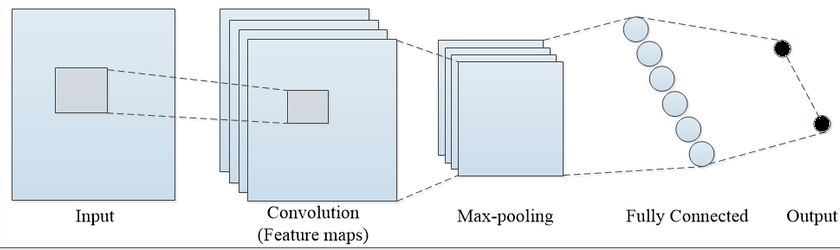
\includegraphics[width=12cm]{convo}
	\caption{CNN Architecture source: \cite{lecun1995convolutional}}
	\label{fig:convo}
\end{figure}

\newpage
\subsection{Relevant Architectures}
\begin{flushleft}
There are many different ways by which to structure the different layers of a CNN, and this section will serve to outline some important CNN architectures that are commonly used. These architectures will later be implemented and investigated during the Empirical Studies section.
\end{flushleft}

\subsubsection*{MobileNet}
\begin{flushleft}
Following the success of AlexNet in 2012, CNN's followed a general trend towards deeper and more computationally expensive architectures. However, increased network complexity does not guarantee increased network performance (\cite{szegedy2016rethinking}), and in computationally limited platforms such as smartphones and self-driving cars tasks need to be carried out quickly with a low computational overhead. The MobileNet architecture arose out of this demand for more lightweight and efficient architectures (\cite{howard2017mobilenets}). MobileNet differs from conventional CNN architectures in that it makes use of depthwise seperable convolutions in the place of regular convolutions. A depthwise seperable convolution consists of two operations - a depthwise convolution that filters through the input image followed by a pointwise (simply 1x1) convolution which combines the outputs of the former. This depthwise seperable convolution serves the same purpose as a traditional convolution, however it is much faster (\cite{howard2017mobilenets}).
\end{flushleft}

\subsubsection*{Inception}
\begin{flushleft}
In a similar vein to the MobileNet architecture, the Inception architecture arose from a desire to create more complex networks to increase performance, without leading to the issues presented by simply stacking more layers into a  network. At the current time there are four main versions of the Inception architecture, with each improving slightly over the preceding version. The core concept behind the creation of this network was that important objects or regions within a given image can vary greatly depending on the differing distances between the object instances and the camera. Due to this variance, selection of the correct kernel size is difficult (\cite{szegedy2016rethinking}). A larger kernel size is suitable for the larger objects, however this will not suffice for the smaller objects. Rather than simply adding extra layers, a possible solution is to have multiple filters operate on the same level, creating a "wider" rather than "deeper" architecture (\cite{szegedy2016rethinking}). This was the driving concept behind the creation of the first Inception architecture (also known as GoogLeNet).
\end{flushleft}

\subsection{Detection Algorithms}
\begin{flushleft}
An integral part of the performance of any CNN is the particular detection algorithm that the CNN utilises. These algorithms are necessary in order to reduce target images into regions that likely contain instances of objects, rather than attempt object detection upon all regions of the images (\cite{girshick2014rich}). This is required in order to reduce the computational requirements of the CNN. Base networks such as Inception or MobileNet perform high-level detection of objects, while detection algorithms are used to find potential occurences of objects to be detected - thus the two work in tandem. 
\end{flushleft}
\subsubsection*{R-CNN}
\begin{flushleft}
To avoid the problem of simply selecting a huge number of regions (\cite{girshick2014rich}) proposed a method whereby 2000 distinct regions of interest (ROI's) were identified in the input image in what are known as "region proposals", with these being identified based on a selective search algorithm. The CNN then acts upon these ROI's in order to detect objects within the region proposals.
\end{flushleft}

\subsubsection*{Faster R-CNN}
\begin{flushleft}
Following advancements made upon the R-CNN algorithm, the Faster-RCNN algorithm was proposed by (\cite{ren2015faster}). This algorithm involves the target image being provided to a CNN which produces a feature map. The predicted ROI's are then reshaped using a particular pooling layer, following which object detection can take place upon the ROI's. This advancement upon earlier R-CNN algorithms produced an algorithm much faster than previous versions of the algorithm.
\end{flushleft}

\subsubsection*{YOLO}
\begin{flushleft}
YOLO (You Only Look Once) does not utilise regions in an attempt to localise objects. Instead, this algorithm utilises a network that attempts to predict classes and their bounding boxes in a single evaluation (\cite{redmon2016you}), creating a search algorithm that is extremely fast, albeit one that struggles with objects at smaller scales.
\end{flushleft}

\subsubsection*{SSD}
\begin{flushleft}
SSD (Single Shot Detection) operates in a similar manner to YOLO, with ROI's being avoided in favour of a single evaluation. SSD has six feature maps at different sizes, making it more capable than YOLO of detecting objects at differing levels of scale.
\end{flushleft}

\subsection{Evaluating the Classifier}
\begin{flushleft}
There are various techniques which can be used to evaluate the operation of a classifier. Some of the more prevalent ones, many of which will be seen throughout the rest of this report, are explained below.
\end{flushleft}

\subsubsection*{Top-1 and Top-5 Accuracy}
\begin{flushleft}
First, the CNN makes a classification. Then in the case of Top-1, the class of the highest probability is checked against the target label. In the case of Top-5, the target label is compared with the top five highest probability predictions. Following this, in both cases the classifier score is calculated as the number of times that the prediction matched in either Top-1 or Top-5, divided by the total number of data points.
\end{flushleft}

\subsubsection*{Accuracy Issues}

\begin{flushleft}
Generally speaking using accuracy alone (number of correctly labelled classes) is not a very reliable metric for an object detection algorithm. For example, if there were 95 dogs and 5 cats to be classified a classifier may label all objects present as dogs. This would lead to an overall accuracy score of 95\%, however this classifier is obviously quite flawed. This is known as class imbalance, and in real life scenarios tends to be the norm. The decisions reached by the classifier can be explained as follows:

\begin{enumerate}
  \item True positive: a positive example classified as positive
  \item True negative: a negative example classified as negative
  \item False positive: a negative example classified as positive
  \item False negative: a positive example classified as negative
\end{enumerate}

False negatives are particularly an issue for the field of self-driving cars, where this result could have potentially fatal ramifications. An example of a false negative classification was seen during a fatal crash of a Tesla model S in May 2016, whereby the autopilot system failed to recognise a white truck against a clear, brightly lit sky. Thus, we need to do more than just measure accuracy in order to properly evaluate the classifier (\cite{rogers2016first}).
\end{flushleft}

\subsubsection*{Confusion Matrix}
\begin{flushleft}
A Confusion Matrix, also referred to as an Error Matrix, is a relatively simple technique for classifier evaluation. It is essentially a table that plots the number of correct and incorrect predictions for all of the different classes. The false positives, false negatives, true positives and true negatives are plotted then the average value for all classes combined is calculated, as demonstrated in the confusion matrix below.

\begin{table}[ht!]
\begin{tabular}{lllllll}
          &                        & \multicolumn{1}{r}{Actual}           &                                      &  &  &  \\
          &                        & \multicolumn{1}{c}{+}                & \multicolumn{1}{c}{-}                &  &  &  \\ \cline{3-4}
Predicted & \multicolumn{1}{l|}{Y} & \multicolumn{1}{l|}{True Positives}  & \multicolumn{1}{l|}{False Positives} &  &  &  \\ \cline{3-4}
          & \multicolumn{1}{l|}{N} & \multicolumn{1}{l|}{False Negatives} & \multicolumn{1}{l|}{True Negatives}  &  &  &  \\ \cline{3-4}
          &                        &                                      &                                      &  &  &  \\
          &                        &                                      &                                      &  &  & 
\end{tabular}
\caption{Confusion matrix visualised}
\end{table}
\end{flushleft}

\subsubsection*{Other Evaluation Metrics}
\begin{flushleft}
There are a number of different metrics of evaluation that can be used other than accuracy alone, with the major ones being summarised in the section. An important point to note is that each of these metrics is derived from the confusion matrix explained above, and can be thought of as different ways of summarising the matrix.

\vspace{0.5cm}
\textbf{Precision}
\linebreak
The precision is the number of correct positive predictions compared to the actual number of positive examples. It can be represented by the formula $precision = \frac{\#TP}{\#TP + \#FP}$. This is a good metric to evaluate when there is a high cost associated with a false positive. For example, an email spam detector must have high precision in order to avoid mistakenly classifying legitimate emails as spam. 

\vspace{0.5cm}
\textbf{Recall}
\linebreak
The recall is the ratio of correct positive examples to the number of positive predictions, and can be represented as $recall = \frac{\#TP}{\#TP + \#FN}$. Recall is an important metric when there is a high cost associated with false negatives and as mentioned above are an extremely important metric for this project.

\vspace{0.5cm}
\textbf{F-score}
\linebreak
Another metric can be derived from precision and recall, known as F-score. F-score is the harmonic mean of precision and recall, and is defined as 
$F = 2. \frac{precision - recall}{precision + recall}$. The F-score can be thought of as representing the balance between the precision and the recall. Although this is an important metric overall, it does not take precedence in this project, where a good recall score is of utmost importance.
\end{flushleft}

\subsubsection*{AUC-ROC Curve}
\begin{flushleft}
The AUC (Area Under Curve) ROC (Receiver Operating Characteristics) curve is another method of classifier evaluation, enabling the visualisation of results from a classification problem. The ROC curve is used to plot the true positive rate against the false positive rate, resulting in a probability curve, while the AUC represents how well the model distinguishes between classes. The higher the AUC, the better the model is. This is visualised in Fig \ref{fig:aucroc}.
\end{flushleft}

\vspace{0.5cm}
\begin{figure}[ht!]
	\centering
	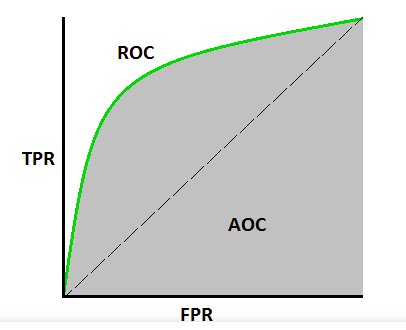
\includegraphics[width=8cm]{aucroc}
	\caption{AUC-ROC Curve (adapted from https://towardsdatascience.com/understanding-auc-roc-curve-68b2303cc9c5)}
	\label{fig:aucroc}
\end{figure}

\newpage
\subsubsection*{Loss}
\begin{flushleft}
As mentioned above, Neural Networks utilise a loss function in order to evaluate the predictions the network makes in relation the known values in the training data. The loss of a network can be graphed to infer how well the model is adjusting to learn the parameters of the training data, with the loss generally lowering over each training iteration.
\end{flushleft}

\subsection{Transfer Learning}
\begin{flushleft}
Transfer learning is a popular technique in Machine Learning whereby an already trained model is retrained on some limited set of new data whilst keeping most of the learned parameters from the original training data. As mentioned earlier, CNN's use their lower layers to extract primitive features such as edges, the middle layers detect shapes from these edges and the final layers learn the task specific abstractions of these shapes. Thus, it is only the final layers that are specific to the classes of the training dataset, with the preceding layers being more general (\cite{yosinski2014transferable}). In transfer learning a base network is trained on a base set of data, after which the learned features of this network are repurposed to a second network which is then trained on the target dataset. In essence, the initial layers of a neural network can be viewed of as feature extractors, and these feature extractors tend to be quite versatile across different datasets (\cite{tan2018survey}). In order for transfer learning to be effective, the original and target datasets must have some degree of similarity in order for the originally learned features to be effective when applied to the target dataset. Transfer learning is a very popular field within Machine Learning, as it can help drastically cut down on training times, as well as enable better results on smaller datasets (\cite{tan2018survey}). The bulk of the experiments carried out in the Empirical Studies section of this report leverage transfer learning in order to cut down on training times.
\end{flushleft}

\section{Berkeley Deep Drive}
\subsubsection{Dataset}
\begin{flushleft}
As mentioned previously in this report, the dataset utilised for this project is the Berkeley Deep Drive dataset, a "large-scale diverse driving video dataset", also known as the BDD100K dataset. Released in 2018, the dataset consists of 100,000 1280x720 annotated images and 100,000 720p 30fps video sequences (\cite{yu2018bdd100k}). The video was collected from a number of locations throughout the United States and consists of a range of weather conditions including sunny, overcast, and rainy. The data consists of a mixture of both daytime and nighttime driving conditions. The images section of the dataset has been created by selecting and annotating the frame at the 10th second of every video. Annotated objects range across 10 different classes - bus, light, sign, person, bike, truck, motor, car, train and rider. The number of instances of each of these annotations are displayed in Fig \ref{fig:annotations}.
\end{flushleft}

\vspace{0.5cm}
\begin{figure}[ht!]
	\centering
	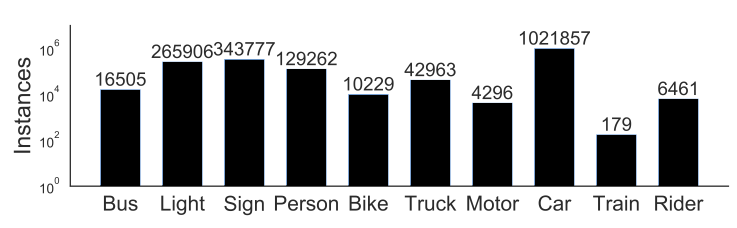
\includegraphics[width=12cm]{annotations}
	\caption{source: https://bair.berkeley.edu/blog/2018/05/30/bdd/}
	\label{fig:annotations}
\end{figure}

\subsubsection{Related Results}
\begin{flushleft}
The paper released with the BDD100K dataset contains a list of results from experiments carried out on the dataset. The experiments focused on the performance of a CNN on different domains within the dataset. For example, a Faster-RCNN was trained on daytime images and then its performance on nighttime images was tested and the discrepancies recorded. The performance metrics recorded from these experiments allow some basis upon which the CNN's trained in this project can be evaluated against. Across the three main classes that will be focused upon in later sections of this report - car, traffic light and person - Yu et al. achieved a mean average precision (mAP) of 0.53. Unfortunately, this is the only metric by which their model was evaluated, however this still provides a rough estimation of how classifiers implemented in later sections should aim to perform.
\end{flushleft}

\section{Overfitting}
\begin{flushleft}
An important point to consider when training any Machine Learning model is how well the model generalises to new data (\cite{domingos2012few}). An algorithm should be able to apply concepts learned from the training data to any previously unseen data in the problem domain in order to make accurate predictions. Overfitting is the concept of a model learning the details and noise in the training domain too well, and thus failing to provide accurate predictions on new data. Overfitting tends to occur when a model learns noise and randomness in the training data as concepts that it attempts to apply to data in the problem domain. These concepts will not apply to the new data however, and poor accuracy generally results. Although a noisy dataset will increase the severity of overfitting, it is not simply a result of a noisy dataset and can occur in any dataset (\cite{domingos2012few}). Within the field of Neural Networks, a common approach to avoid severe overfitting is to keep the network architecture relatively simple. The less parameters required to train the model, the lower the overall chance that the network will overfit and fail to generalise (\cite{o2015introduction}). However, this approach is not always feasible when dealing with large and complex datasets, and other approaches must also be taken. Another popular method to reduce overfitting is the introduction of dropout in the network. Dropout is when nodes are randomly dropped from the network along with their connections (\cite{srivastava2014dropout}). This serves to constrain the adaptation of the network while it trains in order to prevent the model from over-learning the training data.
\end{flushleft}

\section{Tensorflow Introduction and Environment Setup}

This section is dedicated to the background work done in order to gain an understanding of how to implement CNN's using tensorflow. The experiments illustrated in this section were carried out during the completion of the Complete Guide to TensorFlow for Deep Learning with Python course on Udemy (\cite{udemy}). This section consists of two experiments carried out on the MNIST and CIFAR-10 datasets. The first experiment is sample code provided as part of the course to illustrate the concepts learned during the course. The second experiment is an exercise for the course carried out to implement an understanding of these concepts.

\subsection{MNIST Experiment}

The first experiment carried out was the implementation of a very simple CNN. The architecture of the CNN consisted of two layers of Convolution, two pooling layers and a fully-connected layer. After carrying out 5000 training steps with a batch size of 50, a final Top-1 accuracy of 98.75\% was achieved.

\subsubsection*{Code Breakdown}

\begin{flushleft}
The functions displayed in Figure \ref{fig:helpers} are all helper functions. The init\_weights function initialises the random weights for fully connected or convolution layers, with the shape of the layer passed in as a parameter. The init\_bias function performs the same operation for the bias. The conv2d function creates a convolution using a built in function from tensorflow. The max\_pool\_2by2 function creates a max pooling layer, also using built in tensorflow functions. The convolutional\_layer function uses the conv2d function to return an actual convolutional layer with a ReLu activation function. Lastly, the normal\_full\_layer returns a normal fully connected layer.
\end{flushleft}

\vspace{0.5cm}
\begin{figure}[ht!]
	\centering
	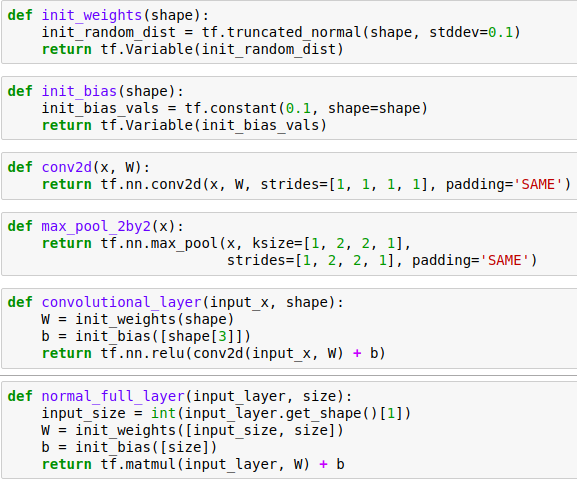
\includegraphics[width=12cm]{helpers}
	\caption{Creating Helper Functions}
	\label{fig:helpers}
\end{figure}

\begin{flushleft}
The functions displayed in Figure \ref{fig:layers} are used to create the convolution and pooling layers of the network. In creating convo\_1, we can see that a 6x6 filter is used from the parameters. An ouput value of 32 is used to represent the number of filters used. The parameter of 1 represents the original input of the image. This carries down to the other layers, with convo\_2 taking in an input image of 32 from convo\_1.
\end{flushleft}

\vspace{0.5cm}
\begin{figure}[ht!]
	\centering
	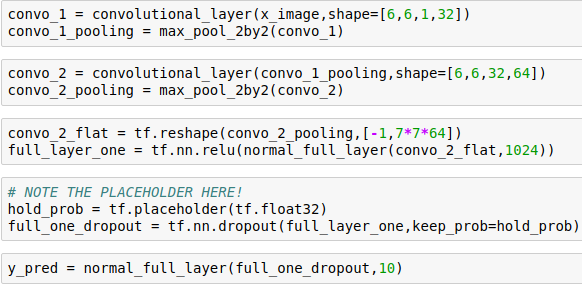
\includegraphics[width=12cm]{layers}
	\caption{Creating Layers}
	\label{fig:layers}
\end{figure}

\begin{flushleft}
The code displayed in Figure \ref{fig:training} shows the model being trained. A tensorflow session is created and data is read in from the dataset. The session is ran to begin model training. The current training step and current error calculated from a loss function is displayed as output as the model trains.
\end{flushleft}

\vspace{0.5cm}
\begin{figure}[ht!]
	\centering
	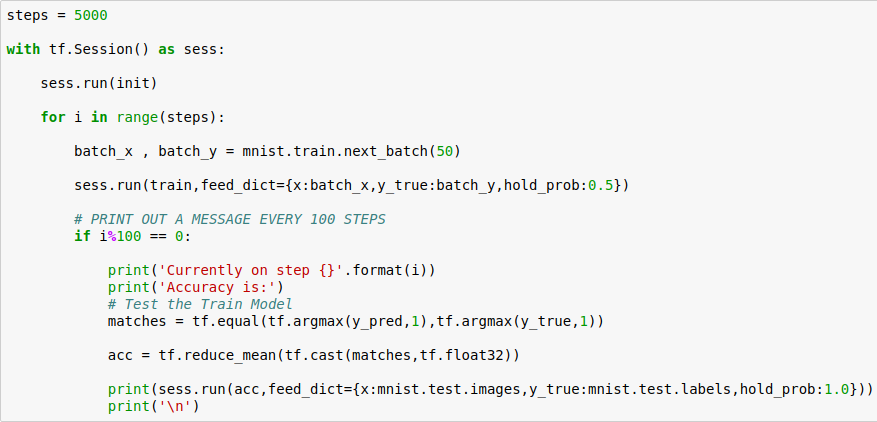
\includegraphics[width=12cm]{training}
	\caption{Training the Model}
	\label{fig:training}
\end{figure}

\newpage
\subsection{CIFAR-10 Experiment}

\begin{flushleft}
The second experiment was carried out on the CIFAR-10 dataset, and the architecture used was consistent with the first experiment, consisting of two layers of Convolution and Pooling. After 5000 training steps with a batch size of 100, a final Top-1 accuracy of 72\% was reached.
\end{flushleft}

\subsection{Initial Findings}

The first two experiments were carried out using CNN's of the same architecture, however an accuracy discrepancy of 26.75\% was observed. Both datasets contain images labelled into 10 classes. The differences arise in the dataset size and image complexity. Firstly, the CIFAR-10 dataset contains 50,000 training images, whereas the MNSIT dataset contains 60,000 training images. The images in the MNSIT dataset are grayscale, whereas images in the CIFAR-10 dataset consist of 3 colour channels. The images in the CIFAR-10 dataset are also of a higher complexity compared to the handwritten digits in the MNIST dataset. The CIFAR-10 images contain more complex real-world images with noisy backgrounds. These disprepancies between the datasets may explain the disprepancies in the accuracy achieved by the classifiers.

\subsection{Environment Setup and Issues}
\begin{flushleft}
Initial environment setup to carry out the above experiments proved quite challenging. During the first attempts at carrying out the experiments, tensorflow was erroneously installed to run using the training machines CPU. This lead to untenable training times for the experiments. Although the training times were not recorded precisely, each experiment took over a day to finish training, during which time the training machine was rendered essentially unusable due to the high load on its CPU. There were two main take-aways from the initial iterations:

\begin{enumerate}
  \item Tensorflow should be installed properly to use the GPU in order to manage training times.
  \item Training times should be recorded for better understanding of the experiments.
\end{enumerate}

\end{flushleft}

\subsubsection{Tensorflow Install}
\begin{flushleft}
The initial attempts to setup tensorflow were carried out on a machine running Windows 7. These attempts failed due to a broken version of Bazel, the build tool used to compile tensorflow. These issues were solved via downgrading to an earlier version of Bazel, however new versioning issues were then encountered due to CUDNN, Nvidias GPU-accelerated library for deep learning. Several different versions were installed without success. Due to these issues seemingly being exclusive to Windows, it was decided to attempt an install on a different machine running Ubuntu. The tensorflow install for the Ubuntu machine was carried out without issue. All neccessary Nvidia drivers were installed on the system, and tensorflow was then installed and the experiments were carried out again. The training times for running the two experiments with GPU acceleration were 12 and 16 minutes respectively, a vast improvement over the initial times. The GPU on the Ubuntu machine was an Nvidia Geforce GTX 650 with 2GB memory.
\end{flushleft}

\subsubsection{Memory Issues}
\begin{flushleft}
Although the first two experiments ran without issues, problems were quickly encountered when modifications were made to the Cifar-10 experiment. In an attempt to improve accuracy results, two further layers of convolution and pooling were added. This led the out of memory (OOM) errors being thrown during training. This was caused by the graphical memory on the training machine being maxed out at the full 2GB. Several attempts at rectifying the issues were carried out. The first attempt tried was reduction of batch size from 100 images, causing less of the dataset being loaded into memory. At a batch size of 4 images, the three layer network successfully trained. The issue with this approach however is that a smaller batch size causes the gradient estimate of the network to be less accurate, and Top-1 accuracy of the network dropped to 60.46\%. The second approach was to simply keep the number of layers low, resulting in a simpler network with less memory requirements. Both of these solutions were not viable for this project. Poor accuracy scores and an inability to train complex networks created an obvious demand for a more powerful training machine. Another point to note is image size disparities between the Cifar-10 dataset and the overall target dataset for this project, the Berkeley Deep Drive dataset. A machine struggling with the 32x32 low resolution images of the Cifar-10 dataset would surely run into a host of issues with the 1280x720 images of the target dataset. As such, it was decided that a much more advanced machine would be required. It was decided that utilising Amazon Web Services (AWS) products was the only way to quickly and easily access the required computational power demanded by this project.
\end{flushleft}

\subsubsection{AWS Setup}
\begin{flushleft}
One of the many services offered by the AWS platform are Amazon Machine Images (AMI) for Deep Learning. These are virtual machine instances that launch with pre-installed pip deep learning frameworks such as tensorflow, keras etc. in different environments, as well as GPU acceleration. This allows development of models remotely from a client machine which can be then trained using the available GPU resources on the deep learning instance. These instances can be deployed and the desired environment (tensorflow in this case) activated. Jupyter notebooks can be run as normal on the AWS instance, and a rule is set up on the client machine to forward all requests on a certain port to the AWS instance. This allows the user to write code in a Jupyter notebook remotely on the AWS instance. The instance type chosen for this project was the p2.xlarge instance which contains 122GiB of memory, 16 virtual CPU cores and a Nvidia K80 GPU. This instance is the cheapest GPU accelerated instance type available, as this project has been funded out of pocket on a tight budget. Costs for these machines are based on usage, so every hour that the machine is running costs are incurred. Much more computationally powerful instances are available, however the costs for these increase dramatically and were not within budget for this project. The steps followed for setting up the instance were from the official AWS documentation (\cite{aws}).
\end{flushleft}

\chapter{Cifar-10 Further Experimentation}
\begin{flushleft}
Once an AWS Deep Learning machine had been set up to enable investigation into more complex CNN architectures, further experiments were carried out on the Cifar-10 dataset in an attempt to improve the disappointing initial results from the experiments carried out as part of the (\cite{udemy}) tutorial. The base code provided as part of the tutorial was modified in a range of different ways in order to maximise results. In order to evaluate the network properly the following metrics were recorded:

\begin{enumerate}
  \item Peak Top-1 accuracy
  \item Precision
  \item Recall
  \item Training time
\end{enumerate}

The baseline of these metrics achieved by the simple network provided from the tutorial are shown in the table below, with the accuracy, precision and recall being graphed in Fig \ref{fig:baseline}. Interestingly enough, the accuracy and recall values for this experiment were identical throughout all of the training steps. This means that the model is somehow "balanced", in that it correctly classifies positive examples at the exact rate that it classifies negative examples. This does not necessarily mean that there is an issue, however it is very unusual. A focus for the following experiments was to investigate what changes, if any, would cause these values to diverge.
\end{flushleft}

\vspace{0.5cm}
\begin{table}[ht!]
\begin{tabular}{llll}
\\ \hline
\multicolumn{1}{|l|}{Peak Top-1 accuracy} & \multicolumn{1}{l|}{Training Time} & \multicolumn{1}{l|}{Precision} & \multicolumn{1}{l|}{Recall}  \\ \hline
\multicolumn{1}{|l|}{70.16\%}             & \multicolumn{1}{l|}{220s}          & \multicolumn{1}{l|}{71.67\%}   & \multicolumn{1}{l|}{70.16\%} \\ \hline
\end{tabular}
\caption{Results from Initial Experiment}
\end{table}

\vspace{0.5cm}
\begin{figure}[ht!]
	\centering
	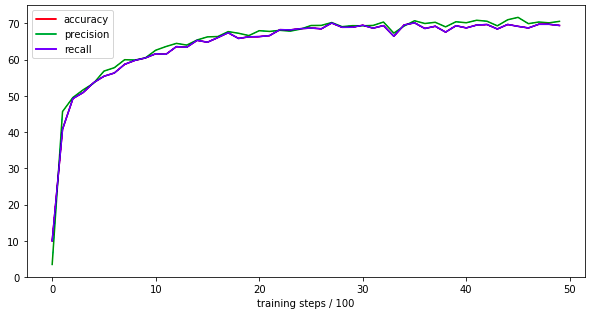
\includegraphics[width=12cm]{baseline-graph}
	\caption{Baseline Plot}
	\label{fig:baseline}
\end{figure}

\begin{flushleft}
\vspace{0.5cm}
\section{Experiment 1: Training Steps}
Before investigating the effects of altering the network architecture, the optimal number of training steps was investigated. This parameter was investigated first as it has a large effect on training time. A network that does not have enough training steps will underlearn, whereby it does not learn all possible parameters. However having too many training steps will lead to increased training time with no increase in accuracy. The initial experiment carried out 5000 training steps, so this was doubled to 10,000 steps in an attempt to see if this would boost accuracy, precision and recall. The results are displayed in the table below and plotted in Fig \ref{fig:experiment-1}. All three metrics levelled off at around the 5000 step mark, with no significant increases reported. It would therefore appear that 5000 training steps is the optimal value.

\vspace{0.5cm}
\begin{table}[ht!]
\begin{tabular}{llll}
\\ \hline
\multicolumn{1}{|l|}{Peak Top-1 accuracy} & \multicolumn{1}{l|}{Training Time} & \multicolumn{1}{l|}{Precision} & \multicolumn{1}{l|}{Recall}  \\ \hline
\multicolumn{1}{|l|}{70.46\%}             & \multicolumn{1}{l|}{466s}          & \multicolumn{1}{l|}{70.71\%}   & \multicolumn{1}{l|}{70.46\%} \\ \hline
\end{tabular}
\caption{Results from Experiment 1}
\end{table}

\vspace{0.5cm}
\begin{figure}[ht!]
	\centering
	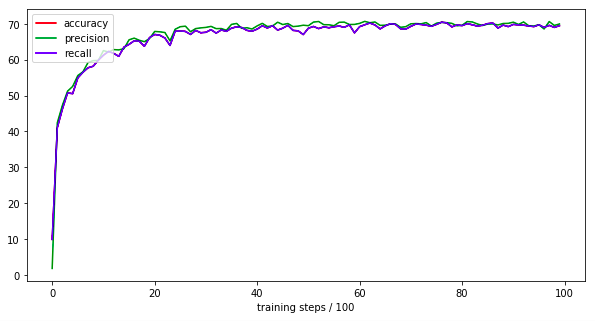
\includegraphics[width=12cm]{experiment-1}
	\caption{10,000 Training Steps}
	\label{fig:experiment-1}
\end{figure}
\end{flushleft}

\begin{flushleft}
\vspace{0.5cm}
\section{Experiment 2: Convolution and Pooling Layers}
The next experiment undertaken was to increase the number of convolution and pooling layers. For this experiment only one extra layer of convolution and pooling was added. As can be shown in the results displayed in the table below as well in Fig \ref{fig:experiment-2}, this did not yield any significant results.

\vspace{0.5cm}
\begin{table}[ht!]
\begin{tabular}{llll}
\\ \hline
\multicolumn{1}{|l|}{Peak Top-1 accuracy} & \multicolumn{1}{l|}{Training Time} & \multicolumn{1}{l|}{Precision} & \multicolumn{1}{l|}{Recall}  \\ \hline
\multicolumn{1}{|l|}{70.38\%}             & \multicolumn{1}{l|}{192s}          & \multicolumn{1}{l|}{70.82\%}   & \multicolumn{1}{l|}{70.38\%} \\ \hline
\end{tabular}
\caption{Results from Experiment 2}
\end{table}

\vspace{0.5cm}
\begin{figure}[ht!]
	\centering
	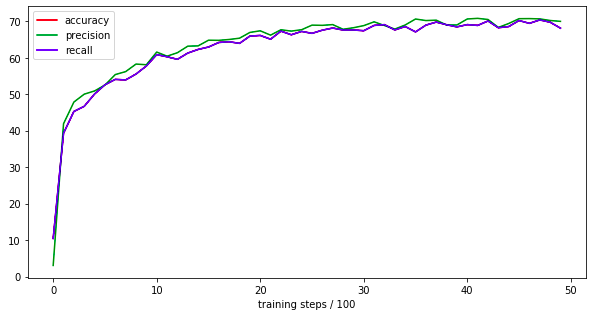
\includegraphics[width=12cm]{experiment-2}
	\caption{Experiment 2}
	\label{fig:experiment-2}
\end{figure}
\end{flushleft}

\begin{flushleft}
\vspace{0.5cm}
\section{Experiment 3: Fully Connected Layers}
As the extra layers of convolution and pooling had failed to yield any benefits, the next step taken was to increase the number of fully connected layers in the network. One extra fully connected layer was added as well as a dropout layer. The reasoning behind this experiment was to investigate the possibility that the network was performing poorly with the class predictions. The images in the Cifar-10 dataset consist of non-occluded blurred objects with one class of object present per image. As such it was reasoned that only a small number of convolution and pooling layers were required to extract feature maps from the images, and increased numbers of fully-connected layers would be more important. Dissapointingly, the results of this experiment were a marginal drop in accuracy, precision and recall.

\vspace{0.5cm}
\begin{table}[ht!]
\begin{tabular}{llll}
\\ \hline
\multicolumn{1}{|l|}{Peak Top-1 accuracy} & \multicolumn{1}{l|}{Training Time} & \multicolumn{1}{l|}{Precision} & \multicolumn{1}{l|}{Recall}  \\ \hline
\multicolumn{1}{|l|}{69.52\%}             & \multicolumn{1}{l|}{161s}          & \multicolumn{1}{l|}{69.67\%}   & \multicolumn{1}{l|}{69.52\%} \\ \hline
\end{tabular}
\caption{Results from Experiment 3}
\end{table}

\vspace{0.5cm}
\begin{figure}[ht!]
	\centering
	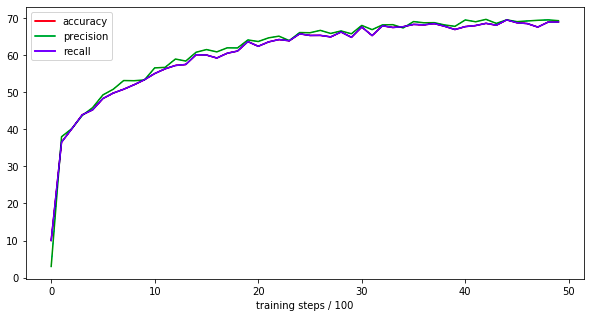
\includegraphics[width=12cm]{experiment-3}
	\caption{Experiment 3}
	\label{fig:experiment-3}
\end{figure}
\end{flushleft}

\newpage
\begin{flushleft}
\vspace{0.5cm}
\section{Experiment 4: Convolution, Pooling and Fully Connected Layers}
As Experiments 2 and 3 had failed to yield better results, 2 extra layers of convolution and pooling were added in conjunction with an extra fully-connected layer. As can be seen from the results table and Fig \ref{fig:experiment-4}, results actually went down marginally.

\vspace{0.5cm}
\begin{table}[ht!]
\begin{tabular}{llll}
\\ \hline
\multicolumn{1}{|l|}{Peak Top-1 accuracy} & \multicolumn{1}{l|}{Training Time} & \multicolumn{1}{l|}{Precision} & \multicolumn{1}{l|}{Recall} \\ \hline
\multicolumn{1}{|l|}{67.3\%}              & \multicolumn{1}{l|}{276s}          & \multicolumn{1}{l|}{68.56\%}   & \multicolumn{1}{l|}{67.3\%} \\ \hline
\end{tabular}
\caption{Results from Experiment 4}
\end{table}

\vspace{0.5cm}
\begin{figure}[ht!]
	\centering
	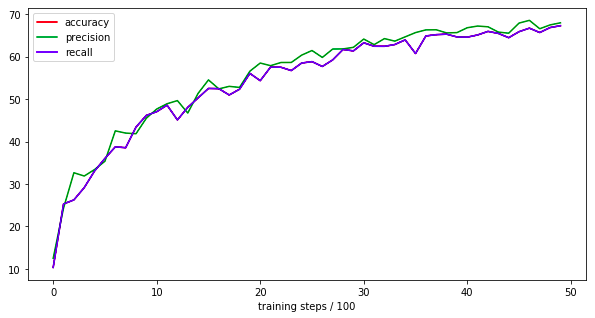
\includegraphics[width=12cm]{experiment-4}
	\caption{Experiment 4}
	\label{fig:experiment-4}
\end{figure}
\end{flushleft}

\newpage
\begin{flushleft}
\vspace{0.5cm}
\section{Experiment 5: Extra Dropout Layers}
Following the failure of experiment 4 to improve results, 2 extra layers of dropout with a probability of 0.25 were added to the experiment 4 architecture after the 2nd and 4th pooling layers in an attempt to tale any potential overfitting. Although the results summarised in the table below and Fig \ref{fig:experiment-5} do not show any meaningful increase in accuracy either, the accuracy curve from this experiment as well as experiment 4 suggest that the network is underlearning as the curves do not level off as much as in previous results. This implied that the network may simply need more time to train. Interestingly, during this experiment the accuracy and recall metrics diverged from one another, as can be observed in Fig \ref{fig:experiment-5}. This would seem to imply that the network may have been overfitting slightly.

\vspace{0.5cm}
\begin{table}[ht!]
\begin{tabular}{llll}
\\ \hline
\multicolumn{1}{|l|}{Peak Top-1 accuracy} & \multicolumn{1}{l|}{Training Time} & \multicolumn{1}{l|}{Precision} & \multicolumn{1}{l|}{Recall}  \\ \hline
\multicolumn{1}{|l|}{60.47\%}             & \multicolumn{1}{l|}{425s}          & \multicolumn{1}{l|}{60.60\%}   & \multicolumn{1}{l|}{60.57\%} \\ \hline
\end{tabular}
\caption{Results from Experiment 5}
\end{table}

\vspace{0.5cm}
\begin{figure}[ht!]
	\centering
	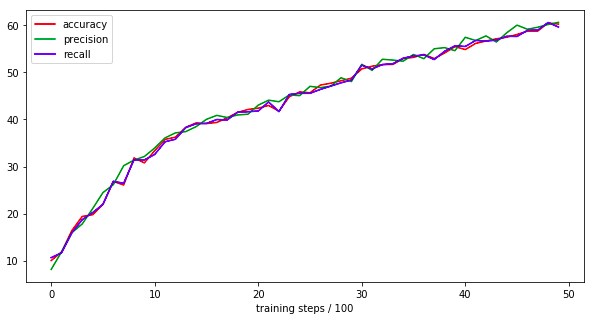
\includegraphics[width=12cm]{experiment-5}
	\caption{Experiment 5}
	\label{fig:experiment-5}
\end{figure}
\end{flushleft}

\clearpage
\begin{flushleft}
\vspace{0.5cm}
\section{Experiment 6: Increased Training Steps}
The observations in experiments 4 and 5 suggested that the network might simply need more time to train. In experiment 1 it was concluded that 5000 training steps would be sufficient, however this experiment was carried out using the simple baseline network architecture. It was therefore a mistake to assume that 5000 training steps would be sufficient for all following experiments. The number of training steps was increased drastically to 25,000, with the architecture remaining the same as in experiment 5. Although training time was significantly increased, all metrics gained a slight increase with accuracy peaking at 73.25\%, a decent improvement from the initial results.

\vspace{0.5cm}
\begin{table}[ht!]
\begin{tabular}{llll}
\\ \hline
\multicolumn{1}{|l|}{Peak Top-1 accuracy} & \multicolumn{1}{l|}{Training Time} & \multicolumn{1}{l|}{Precision} & \multicolumn{1}{l|}{Recall}  \\ \hline
\multicolumn{1}{|l|}{73.54\%}             & \multicolumn{1}{l|}{1778s}         & \multicolumn{1}{l|}{74.03\%}   & \multicolumn{1}{l|}{73.48\%} \\ \hline
\end{tabular}
\caption{Results from Experiment 6}
\end{table}

\vspace{0.5cm}
\begin{figure}[ht!]
	\centering
	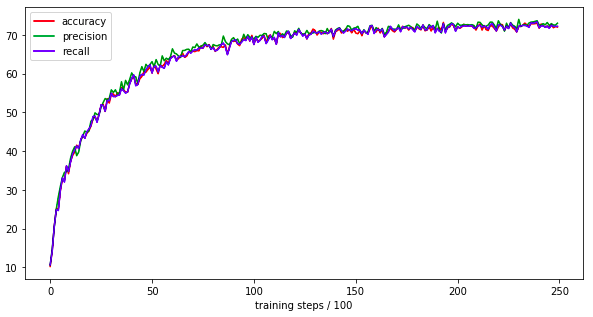
\includegraphics[width=12cm]{experiment-6}
	\caption{Experiment 6}
	\label{fig:experiment-6}
\end{figure}

\end{flushleft}

\begin{flushleft}
\vspace{0.5cm}
\section{Conclusions}
These experiments conclude with a small yet significant increase in accuracy, precision and recall scores from the final experiment, with the results being collated in Table \ref{cifar-results}. These experiments were focused mainly upon the effects of network architecture rather than the effects of parameter tuning. Empirical studies in later sections will focus more on the effects of parameter tuning. Adding just extra layers of convolution and pooling without adding extra fully-connected layers did not result in improvements, and vice versa. Upon creation of a more complex network architecture with dropout layers results actually went down slightly. However, observation of the metric graphs showed that the network was possibly underlearning, and a drastic increase in training steps led to positive results. Accuracy, precision and recall all seemed to increase in proportion with one another for these experiments, however this is generally not guaranteed for all networks. Datasets containing more classes or high levels of class imbalance would typically not result in such regular accuracy, precision and recall metrics. If there is anything to take from these experiments moving forward with this project, it is that simply adding one or two extra layers is not sufficient to gain satisfactory results - adding multiple layers of convolution, pooling and fully-connected layers should be investigated in conjunction with each other in future experiments. As the unusual accuracy and recall results also demonstrate, it may also be beneficial to introduce dropout or some other form of regularisation in networks that are not obviously overfitting. Although the increases in performance shown are slight, I am confident that further increasing the complexity of the network and increasing training times can lead to further increases.
\end{flushleft}

\begin{table}[th!]
\begin{tabular}{|l|l|l|l|l|}
\hline
Experiment no. & Peak Top-1 Accuracy & Training Time & Precision & Recall  \\ \hline
1              & 70.46\%             & 466s          & 70.71\%   & 70.46\% \\ \hline
2              & 70.38\%             & 192s          & 70.82\%   & 70.38\% \\ \hline
3              & 69.52\%             & 161s          & 69.67\%   & 69.52\% \\ \hline
4              & 67.3\%              & 276s          & 68.56\%   & 67.3\%  \\ \hline
5              & 60.47\%             & 425s          & 60.6\%    & 60.57\% \\ \hline
6              & 73.54\%             & 1778s         & 74.03\%   & 73.48\% \\ \hline
\end{tabular}
\caption{Collated results from CIFAR-10 experiments}
\label{cifar-results}
\end{table}

\newpage
\chapter{Empirical Studies}
\begin{flushleft}
The following sections will primarily investigate the effects of retraining various different network architectures using transfer learning. Models were retrained using the Tensorflow Object Detection API, with the steps followed being from a tutorial made available on GitHub (\cite{tutorial}). The main point of note for the Tensorflow Object Detection API is the main config file for each of the experiments. This file defines what type of architecture is used, what pretrained model (if any) is loaded in for retraining and what dataset the model is to be retrained upon. All of the pretrained models utilised in the following sections have been trained on the COCO (Common Objects in Context) dataset, a dataset provided by Microsoft. Although the COCO dataset is updated every year, it currently consists of 164,000 images populated with 90 classes of objects. The dataset was chosen for this project as it contains 8 different classes of vehicle and displays objects in real-life contexts, with potential for occlusion and general variance in the images (\cite{lin2014microsoft}). Many other datasets instead provide an "iconic" view of objects, whereby the object appears centrally and unobstructed in the image. As the BDD100K dataset images are drawn from real-world scenarios from the perspective of a car, using the COCO dataset as the initial training dataset should allow the retrained models to generalise better to the BDD100K data than datasets with less variance in the images. As mentioned in the section related to transfer learning above, it is important that the original training dataset be as closely related as possible to the target dataset (\cite{tan2018survey}).
\end{flushleft}

\section{SSD MobileNet V1 Experiments}
\begin{flushleft}
The MobileNet architecture utilising a SSD detection algorithm was the first architecture selected due to the low computational requirements of this setup.
\end{flushleft}

\subsection{Experiment 1: Full Dataset Retraining}
\subsubsection*{Objectives}
\begin{flushleft}
Initial attempts at retraining the SSD MobileNet V1 were carried out using the full 10k subset of the bdd100k dataset, containing 10,000 images annotated with 10 classes. The objective for this experiment was to retrain the MobileNet model with the new BDD100K data. With training times being a concern when dealing with large datasets, the MobileNet architecture was selected to be retrained first due to its quick training times. This main objective for this first experiment was to investigate how models would handle the large amount of data presented by the BDD100K dataset and to gain some understanding of how the object detection API works. 
\end{flushleft}

\subsubsection*{Setup}
\begin{flushleft}
The tensorflow object detection API only accepts datasets in the tfrecord format, a binary file format for data storage. This requires parsing the images and their labels and writing them into tfrecord format. Luckily, an open source parser for the BDD100K dataset has been made available on GitHub (\cite{parser}). This tool was used to parse all images within the 10k section of the BDD100K dataset, resulting in a tfrecord file containing the data for the full 10,000 images and their annotations.
\end{flushleft}

\subsubsection*{Results}
\begin{flushleft}
After 5000 training steps, the results for this experiment were disappointing albeit not unexpected. As can be seen in Fig \ref{fig:mobilenet-full-dataset-loss}, loss values were extremely high, and did not follow any steady downward trend. Total training time to 10,000 steps took 2 hours and 48 minutes. These poor results were expected due to the very large and highly complex dataset. Fig \ref{fig:noisy} provides an example of this - the nighttime conditions combined with slight motion blur creates a highly variable image on which to make predictions with the classes present within the image being very hard to make out clearly. Notwithstanding dataset variance created by time of day or weather conditions, many of the images in the dataset are complex simply due to the scenes depicted within them. For example, in city scenes rows of cars cause occlusion and people are hard to pick out between the cars. With the dataset consisting in large part of images with similar levels of variance, training times for the full dataset would likely be untenable if a CNN was to be trained to a point where it performed close to the results presented in (\cite{yu2018bdd100k}). A more powerful GPU accelerated machine may have potentially cut down on these training times drastically, however these machines were simply out of budget for this project. As such, investigation into a different approach was required.
\end{flushleft}

\vspace{0.5cm}
\begin{figure}[ht!]
	\centering
	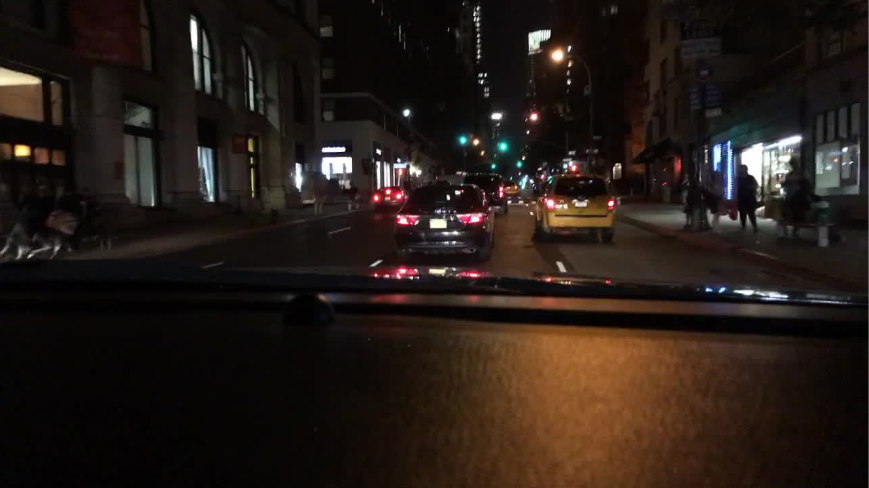
\includegraphics[width=12cm]{noisy}
	\caption{Example of an image that is very hard to annotate}
	\label{fig:noisy}
\end{figure}

\vspace{0.5cm}
\begin{figure}[ht!]
	\centering
	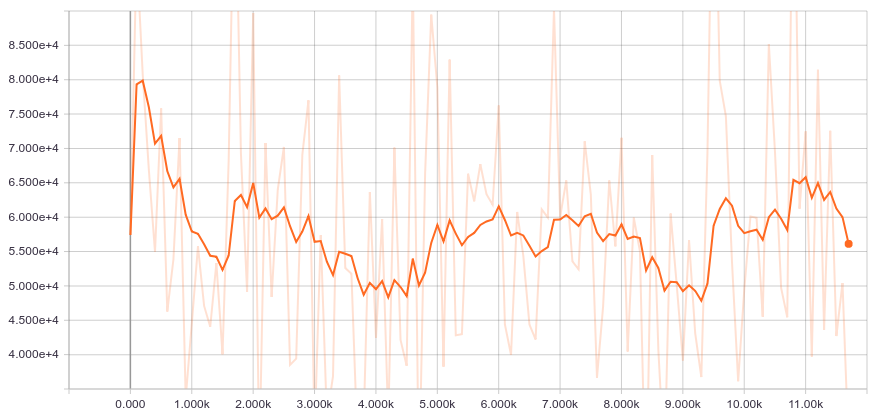
\includegraphics[width=12cm]{mobilenet-full-dataset-loss}
	\caption{Loss values for full dataset}
	\label{fig:mobilenet-full-dataset-loss}
\end{figure}

\newpage
\subsection{Experiment 2: Partial Dataset Retraining}
\subsubsection*{Objectives}
\begin{flushleft}
Following the failure to produce adequate results on the full dataset, it was determined that an approach of drastic data reduction was required in order to investigate training on a problem domain of reduced complexity. The objective for this experiment was therefore to retrain the MobileNet V1 architecture again, this time with a much simpler dataset and with less classes required for detection. In order to achieve this, a subgroup of images would need to be extracted from the dataset and labelled manually.
\end{flushleft}

\subsubsection*{Setup}
\begin{flushleft}
It was determined that 200 total images would be selected to be manually labelled from the bdd100k dataset, with 160 being utilised for training and 40 for testing. Classes labelled for detection were reduced in number to just 3 - cars, traffic lights and people. These classes were chosen as they are commonly present in most images in the dataset and are all unrelated to each other. The images selected were all images taken with good lighting, no motion blur and no inclement weather present. The scenes depicted by the selected images were semi-urban - all three classes were present albeit in lesser numbers for traffic lights and people. Fully urban scenes were avoided due to the potential for extreme levels of class occlusion within the images. The images were annotated using the open source LabelImg tool, before being converted to tfrecord format. Training was then carried out exactly the same as the above experiment, this time with the reduced dataset.
\end{flushleft}

\subsubsection*{Results}
\begin{flushleft}
Although far from perfect, results from this experiment were much more encouraging. As evidenced in Fig \ref{fig:loss-smalldata-5k}, loss quickly declined before settling to values just below 2, with the minimum value being 1.788 and a total training time of just 1hr 25min. Mean average precision (\ref{fig:map-smalldata-5k}) and average recall (\ref{fig:ar-smalldata-5k}), although slighly erratic, appeared to settle into an upward trend as training progressed. Maximum precision reached was 0.1995 and maximum recall reached was just 0.1268. The model can be seen in action at 500 training steps in Fig \ref{fig:class-smalldata-500} and then at 5000 training steps in Fig \ref{fig:class-smalldata-5k}. The improvement in the model is clearly apparent in these two images. Please note however that these images appear blurred due to the fact that this MobileNet architecture was initially trained on images of size 300x300 pixels in order to reduce training times. This means that the BDD100K images that it has been retrained on have been scaled down to size 300x300. Scaling the images back up to full size results in the distortion present in the example images. These results are far from perfect however, and will need to be improved upon. Although the model at 5000 steps detects far more than it did at 500 steps, there are still several of the more occluded cars present in the image not being detected. As mentioned, mean average precision and recall did seem to be improving, however neither value increased to above 0.3, which is comparatively poor results. As such, further experimentation is required.
\end{flushleft}

\vspace{0.5cm}
\begin{figure}[ht!]
	\centering
	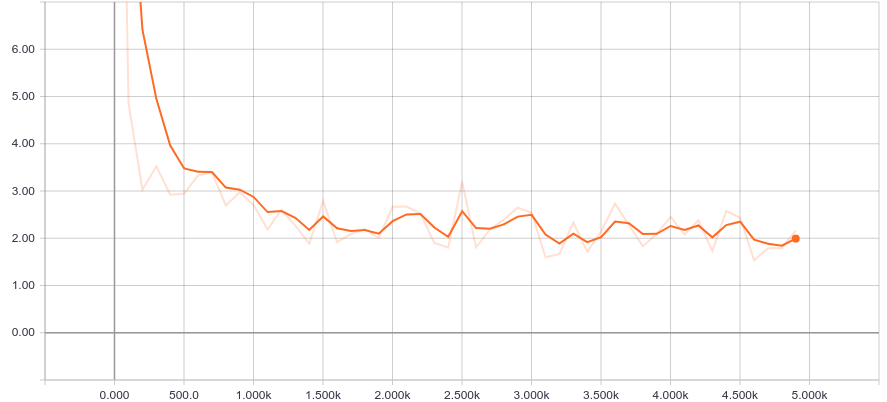
\includegraphics[width=12cm]{loss-smalldata-5k}
	\caption{Loss values for reduced dataset}
	\label{fig:loss-smalldata-5k}
\end{figure}

\vspace{0.5cm}
\begin{figure}[ht!]
	\centering
	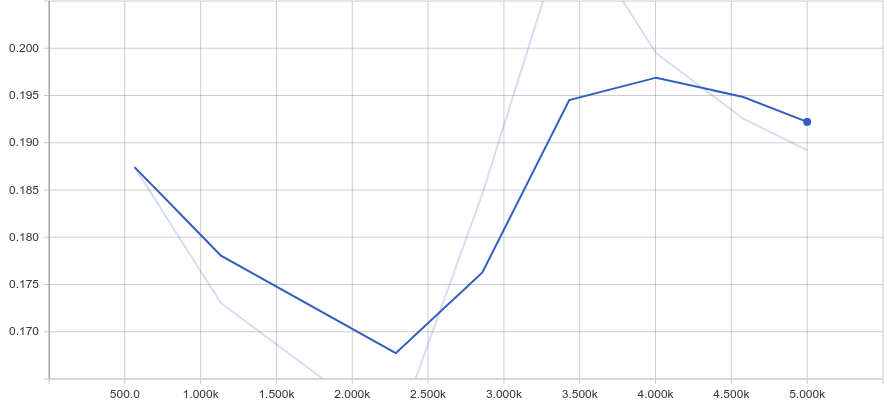
\includegraphics[width=12cm]{map-smalldata-5k}
	\caption{Mean average precision (mAP) values for reduced dataset}
	\label{fig:map-smalldata-5k}
\end{figure}

\vspace{0.5cm}
\begin{figure}[ht!]
	\centering
	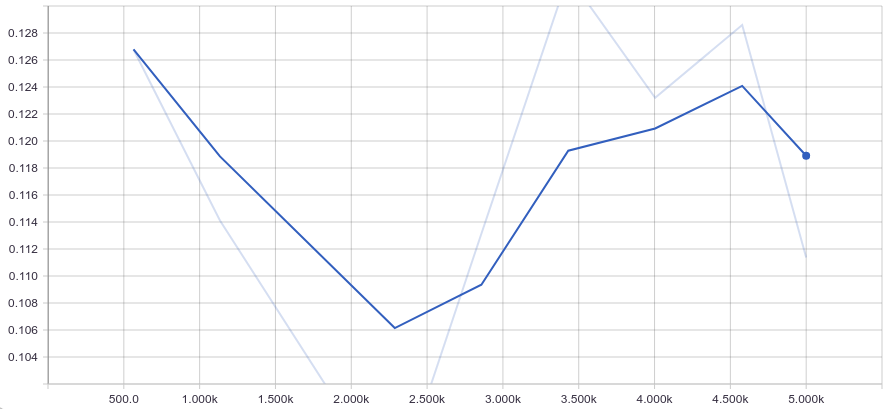
\includegraphics[width=12cm]{ar-smalldata-5k}
	\caption{Average recall (ar) values for reduced dataset}
	\label{fig:ar-smalldata-5k}
\end{figure}

\vspace{0.5cm}
\begin{figure}[ht!]
	\centering
	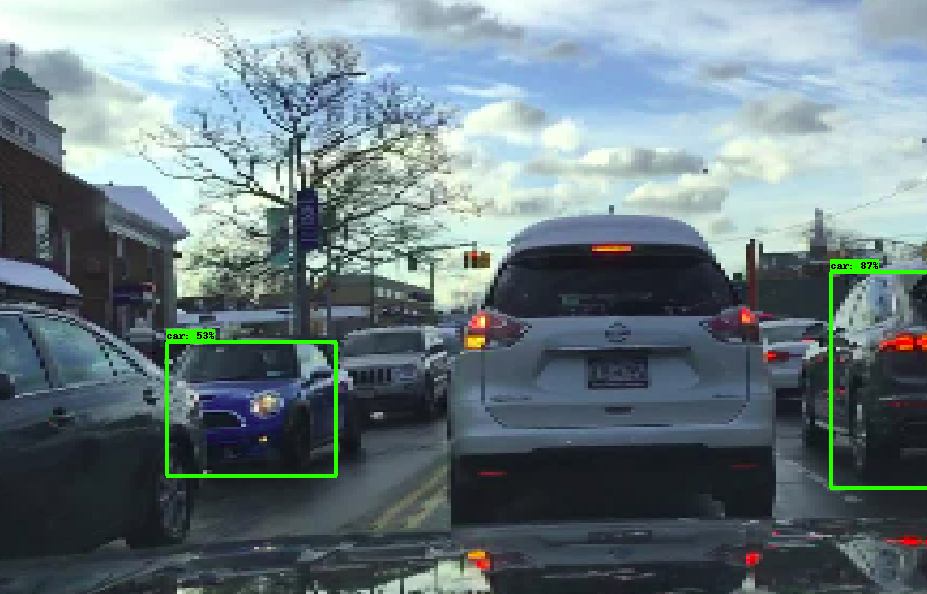
\includegraphics[width=15cm]{class-smalldata-500}
	\caption{Object detector in action at 500 steps}
	\label{fig:class-smalldata-500}
\end{figure}

\vspace{0.5cm}
\begin{figure}[ht!]
	\centering
	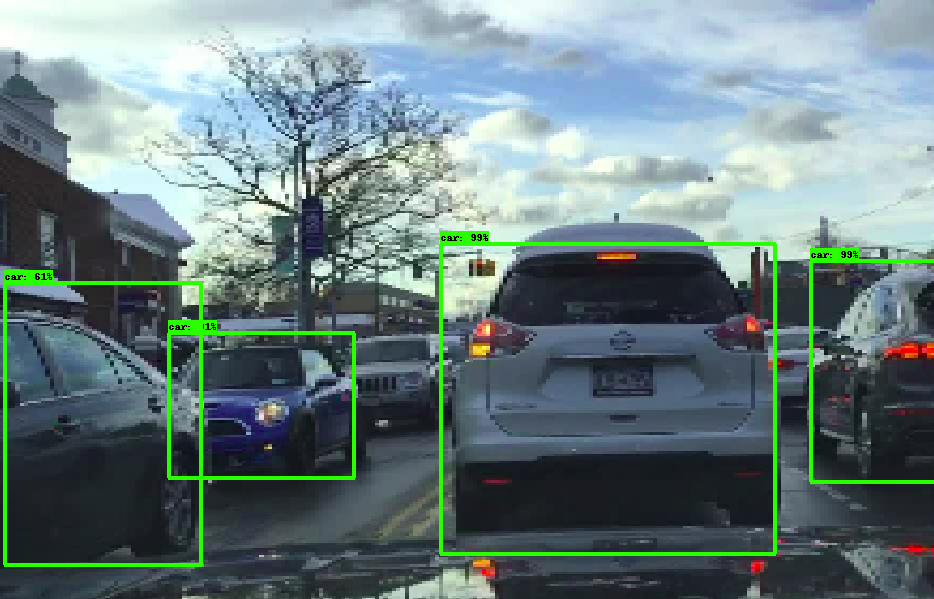
\includegraphics[width=15cm]{classes-smalldata-5k}
	\caption{Object detector in action at 5000 steps}
	\label{fig:class-smalldata-5k}
\end{figure}

\clearpage
\subsection{Experiment 3: Expanded Partial Dataset Retraining}
\subsubsection*{Objectives}
\begin{flushleft}
Following the more encouraging results from the previous experiment, it was decided that the easiest way to boost performance was to simply increase the amount of training data. A further 200 images were hand annotated, with 120 being added to the training data and the final 80 being added to the validation data. This brought the size of the manually annotated dataset to 400 images. Although this is a comparitively small amount, the relatively close relationship between the COCO dataset and the BDD100K dataset was a mitigating factor that allowed a smaller dataset.
\end{flushleft}

\subsubsection*{Setup}
\begin{flushleft}
Setup was carried out almost exactly the same as the previous experiment. 200 total images were annotated manually using LabelImg across the three classes - car, traffic light and person. Images were selected from the same semi-urban scenes without inclement weather or poor lighting. As the dataset had now doubled in size, the number of training steps was increased. The CNN was trained for 14,000 steps, at which point the loss values appeared to not be dropping signicantly.
\end{flushleft}

\subsubsection*{Results}
\begin{flushleft}
Results over the previous experiment were much improved. Over a total training time of 3hr and 50mins to reach 14,000 steps, the loss value fell to a lowest value of 1.356. Precision reached a maximum value of 0.2389 and recall reached a maximum value of 0.1554. Although these results are a significant improvement over the initial experiments, they are still inadequate. Although the MobileNet architecture proved valuable to carry out some initial experiments and highlight the issues presented by the BDD100K dataset it is still unsuitable for this project for several reasons. The requirement to resize the images down to 300x300 pixels in order to provide training images of the same dimensions of the initial COCO training data means that the pretrained MobileNet models provided by tensorflow will never be suitable for achieving acceptable results on the larger BDD100K images, although the MobileNet architecture itself does achieve similar performance to other more complex networks (\cite{howard2017mobilenets}). As such, a different CNN architecture will need to be investigated in order to obtain a trained model that can reliably carry out object detection on the BDD100K dataset.
\end{flushleft}

\vspace{0.5cm}
\begin{figure}[ht!]
	\centering
	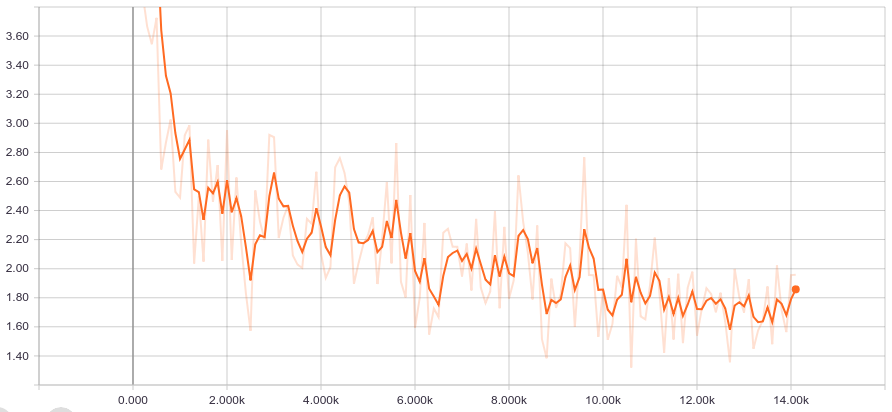
\includegraphics[width=15cm]{loss-mobilenet-2}
	\caption{Loss values for MobileNet with 400 training images}
	\label{fig:loss-mobilenet-2}
\end{figure}

\vspace{0.5cm}
\begin{figure}[ht!]
	\centering
	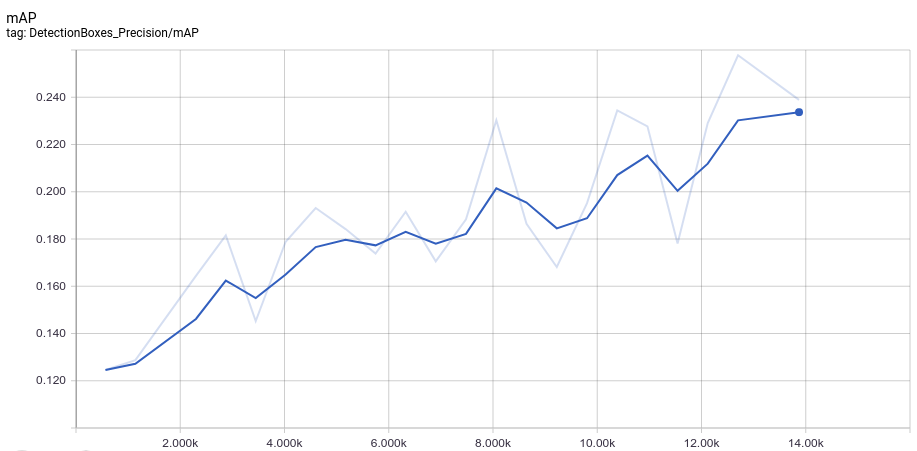
\includegraphics[width=15cm]{precision-mobilenet-2}
	\caption{Precision values for MobileNet with 400 training images}
	\label{fig:precision-mobilenet-2}
\end{figure}

\vspace{0.5cm}
\begin{figure}[ht!]
	\centering
	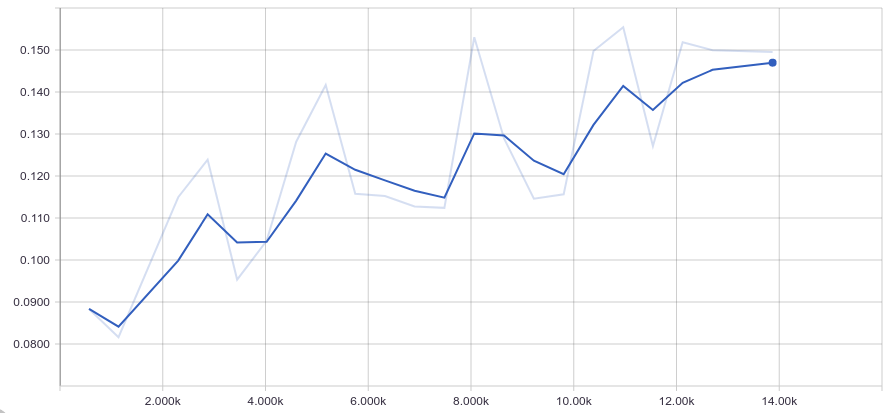
\includegraphics[width=15cm]{recall-mobilenet-2}
	\caption{Recall values for MobileNet with 400 training images}
	\label{fig:recall-mobilenet-2}
\end{figure}

\clearpage
\subsection{Real-time Detection}
\begin{flushleft}
In attempt to discover how suitable the SSD MobileNet model was for detecting objects in real time, the model was applied to video sequences from the BDD100K dataset. As Experiment 3 of this section had produced the best results, the model produced from this experiment was selected. Video sequences were selected from driving conditions that matched those present in the training data. Video sequences were fed into the model frame by frame, where annotation took place frame by frame, producing an output video with objects annotated. Annotation for the model took approximately 0.5 seconds per frame.
\end{flushleft}

\newpage
\section{Faster RCNN Inception V2 Experiments}
\begin{flushleft}
Following the relatively poor results of the MobileNet experiments, the Inception V2 architecture was utilised with a Faster RCNN detection algorithm.
\end{flushleft}

\subsection{Experiment 1: Pretrained Model Experiment}
\subsubsection*{Objectives}
\begin{flushleft}
The objective for this experiment was to retrain the Inception V2 architecture using all of the subsampled data from the BDD100K dataset. As the Inception V2 architecture is a much more complex architecture than the MobileNet architecture, it was expected that the results obtained from this experiment would be much closer to those presented in (\cite{yu2018bdd100k}).
\end{flushleft}

\subsubsection*{Setup}
\begin{flushleft}
Setup for this experiment was minimal as the training data for this experiment had already been annotated. The pretrained Inception V2 model was simply downloaded and the steps presented by (\cite{tutorial}) were once again followed, this time for the new model.
\end{flushleft}

\subsubsection*{Results}
\begin{flushleft}
Results for this experiment were far better than the MobileNet experiments. Over 10,000 training steps taking a total time of 1d 3hr and 25min, loss fell to a minimum value of 0.1253. Precision reached a maximum value of 0.4392 and recall reached a maximum value of 0.2170. The precision score of 0.4392 was a very encouraging result, as this is not drastically different from the results obtained in (\cite{yu2018bdd100k}). These metrics are graphed in Fig \ref{fig:loss-inception}, Fig \ref{fig:precision-inception} and Fig \ref{fig:recall-inception}. As these metrics did not seem to be improving significantly at the 10,000 steps mark, training was halted at this point.
\end{flushleft}

\vspace{0.5cm}
\begin{figure}[ht!]
	\centering
	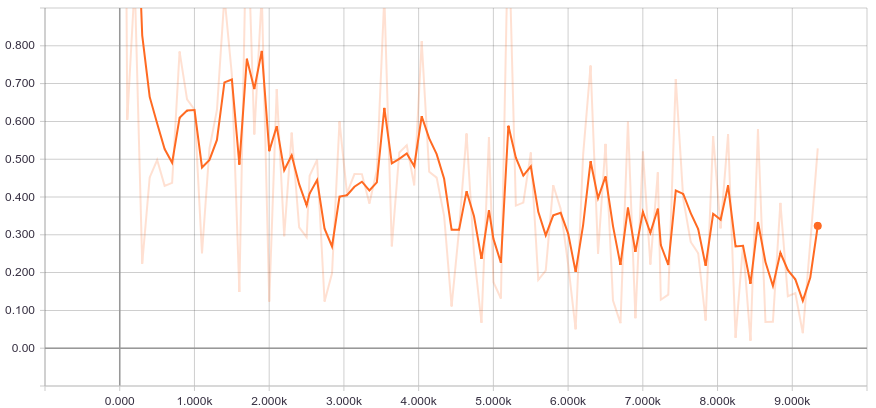
\includegraphics[width=15cm]{loss-inception}
	\caption{Loss values for Inception V2}
	\label{fig:loss-inception}
\end{figure}

\vspace{0.5cm}
\begin{figure}[ht!]
	\centering
	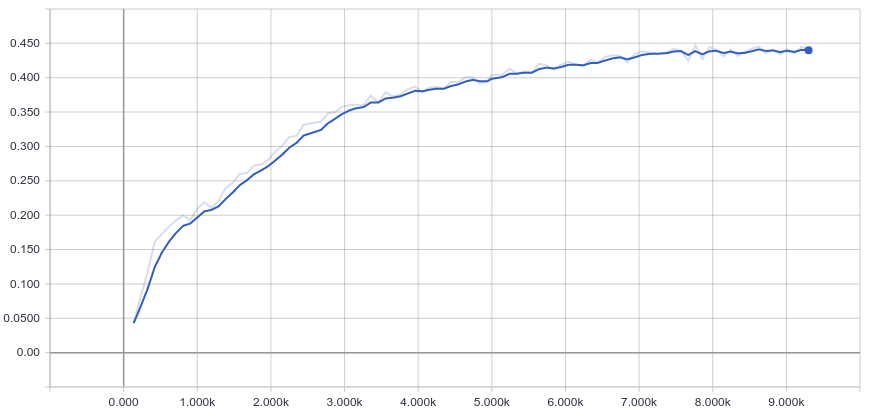
\includegraphics[width=15cm]{precision-inception}
	\caption{Precision values for Inception V2}
	\label{fig:precision-inception}
\end{figure}

\vspace{0.5cm}
\begin{figure}[ht!]
	\centering
	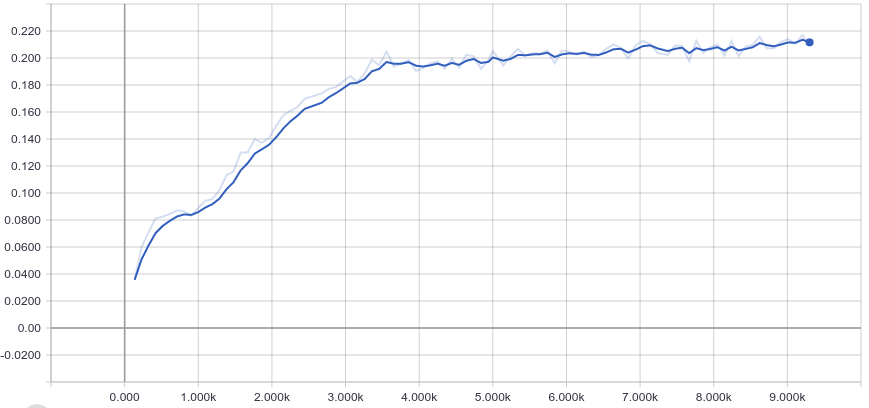
\includegraphics[width=15cm]{recall-inception}
	\caption{Recall values for Inception V2}
	\label{fig:recall-inception}
\end{figure}

\clearpage
\subsection{Experiment 2: No Pretraining Experiment}
\subsubsection*{Objectives}
\begin{flushleft}
As every experiment prior to this experiment was carried out on a pretrained model provided by tensorflow, it was decided to train a model using the Inception V2 architecture that had received no pretraining whatsoever. Results for this experiment were expected to be extremely poor - with a dataset consisting of a meager 400 images overfitting was almost guaranteed.
\end{flushleft}

\subsubsection*{Setup}
\begin{flushleft}
Setup for this experiment was consistent with the previous experiment with one exception - no pretrained model checkpoint was loaded in at the beginning of training.
\end{flushleft}

\subsubsection*{Results}
\begin{flushleft}
As expected, results for this experiment were extremely poor over 3500 training steps totalling 5hr 35 minutes. Although Fig \ref{fig:no-ckpt-loss} may appear to be indicative of positive results, note the fact that this metric is simply the \textit{training} loss. Training any CNN will lead to a lower training loss over time as the CNN adapts and learns the parameters of the training dataset. Observation of the validation loss in Fig \ref{fig:no-ckpt-val-loss}, precision in Fig \ref{fig:no-ckpt-precision} and recall in Fig \ref{fig:no-ckpt-recall} clearly illustrate that this model is severely overfitting. The validation loss does not appear to be following any clear downward trend and although the precision and recall values appear to be following an upward trend, their values are extremely low. This implies that while the model is steadily getting better at detecting objects within the training data, it is failing to achieve these results upon the validation data - a sure sign of a model that is overfitting. Training was halted at 3500 steps as it was clearly apparent that overfitting was taking place and further training would simply be a waste of resources.
\end{flushleft}

\vspace{0.5cm}
\begin{figure}[ht!]
	\centering
	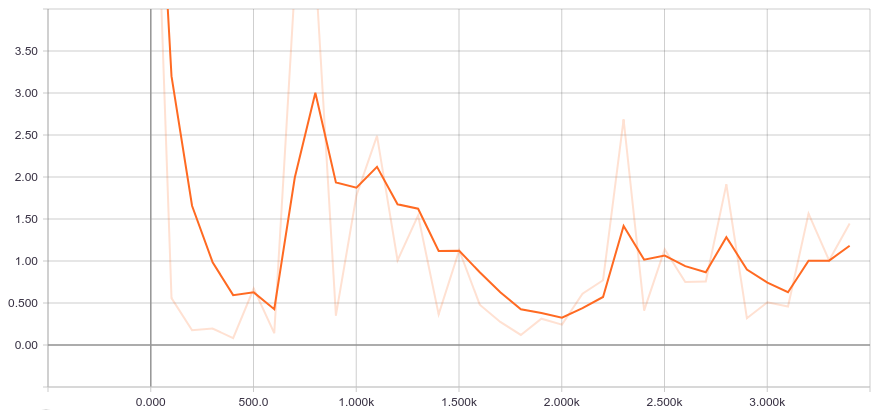
\includegraphics[width=15cm]{no-ckpt-loss}
	\caption{Training Loss with no Pretraining}
	\label{fig:no-ckpt-loss}
\end{figure}

\vspace{0.5cm}
\begin{figure}[ht!]
	\centering
	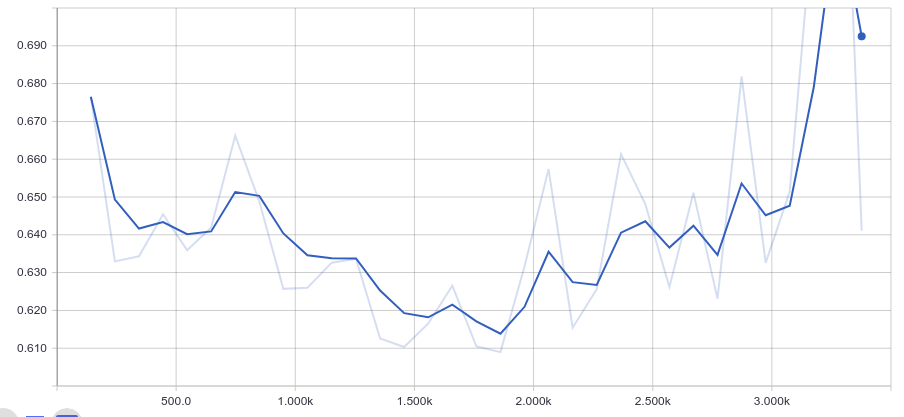
\includegraphics[width=15cm]{no-ckpt-val-loss}
	\caption{Validation Loss with no Pretraining}
	\label{fig:no-ckpt-val-loss}
\end{figure}

\vspace{0.5cm}
\begin{figure}[ht!]
	\centering
	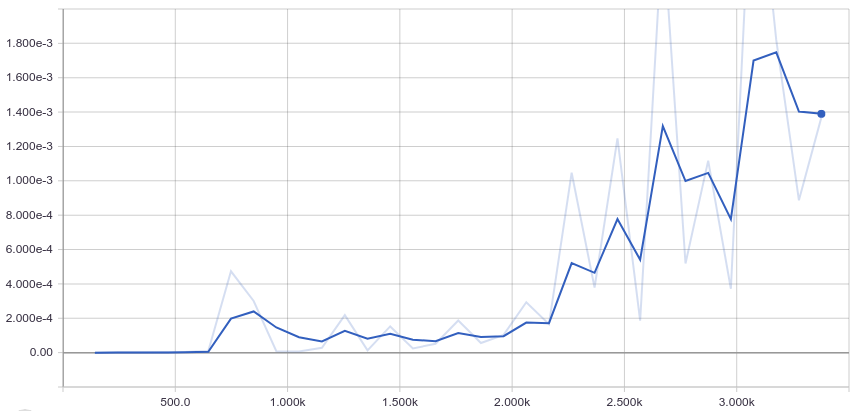
\includegraphics[width=15cm]{no-ckpt-precision}
	\caption{Precision with no Pretraining}
	\label{fig:no-ckpt-precision}
\end{figure}

\vspace{0.5cm}
\begin{figure}[ht!]
	\centering
	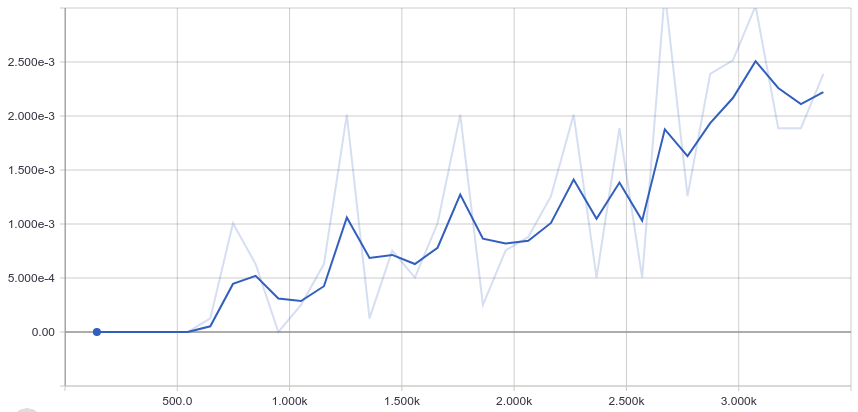
\includegraphics[width=15cm]{no-ckpt-recall}
	\caption{Recall with no Pretraining}
	\label{fig:no-ckpt-recall}
\end{figure}

\clearpage
\subsection{Real-time Detection}
\begin{flushleft}
In attempt to discover how suitable the Faster RCNN Inception architecture was for performing real-time detection, the model from Experiment 1 of this section was utilised for performing video annotation. Although this experiment had achieved much better results than any of the MobileNet experiments, annotation took approximately 3 seconds per frame - a significant increase over the MobileNet experiments. This level of performance would be entirely unacceptable for any potential real-world solution, and it appears that a middle-ground should be investigated, with a solution retaining some of the speed of the SSD MobileNet experiments whilst also retaining some of the evaluation metrics of the Faster-RCNN Inception experiments. A sample video has been uploaded to YouTube to demonstrate how the model behaves in the context of a video and can be viewed at: \href{https://youtu.be/vLHHTuWw1Vw}{https://youtu.be/vLHHTuWw1Vw}
\end{flushleft}

\newpage
\newpage
\section{Empirical Studies Cost and Results}
\begin{flushleft}
At this point in the Empirical Studies, the bills from AWS had run up to a point where it was no longer feasible for further experimentation to take place. Even though the EC2 instance type being utilised was the cheapest GPU accelerated option, the total bill across the months of February and March totalled \$192.53, with a further \$12.48 estimated bill for April across a total of 123.530 total hours of active instance time. The bill for March, during which the bulk of training was carried out, is shown in Fig \ref{fig:bill}. Due to this project being funded by a very tight student budget, this regrettably forced a halt to any further work using AWS resources. However, at this point enough experimentation had been carried out to form some final conclusions as to what would be necessary to achieve better results upon the BDD100K dataset, which will be discussed in the future work section.
\end{flushleft}

\vspace{0.5cm}
\begin{figure}[ht!]
	\centering
	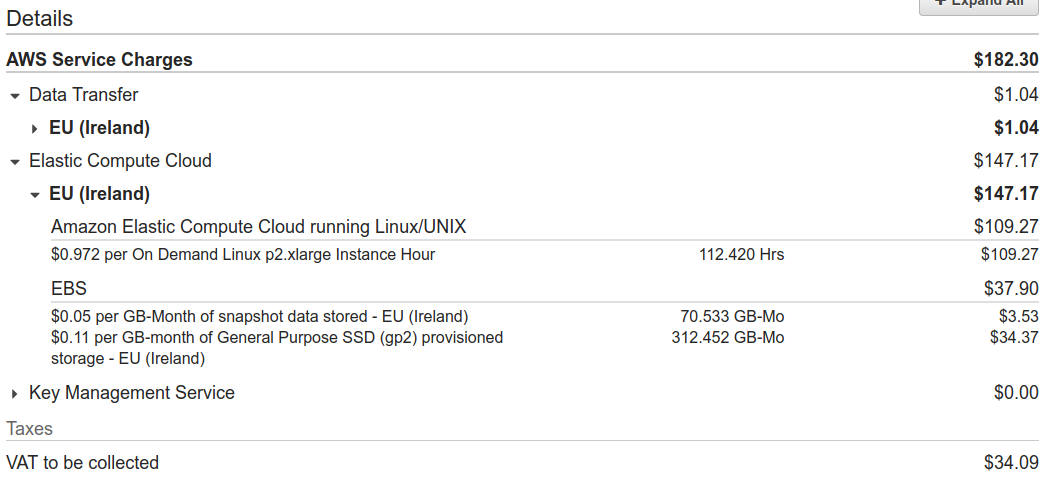
\includegraphics[width=15cm]{bill}
	\caption{AWS Bill for March}
	\label{fig:bill}
\end{figure}

\begin{flushleft}
The results from the Empirical Studies are shown in the below table along with the results provided in (\cite{yu2018bdd100k}). The results from the MobileNet experiment 1 have been omitted as no meaningful results were gleaned from this experiment.
\end{flushleft}

\begin{table}[]
\begin{tabular}[ht]{|p{3cm}|p{2cm}|p{2cm}|p{2cm}|p{2cm}|p{2cm}|}
\hline
Experiment                & Training Steps & Training Time   & Precision  & Recall    & Per-frame annotation \\ \hline
Yu et al.                 & -              & -               & 0.53       & -         & -                    \\ \hline
MobileNet Experiment 2    & 5000           & 1 hr 25 min     & 0.1995     & 0.1268    & 0.5s                 \\ \hline
MobileNet Experiment 3    & 14000          & 3 hr 50 min     & 0.2389     & 0.1554    & 0.5s                 \\ \hline
Inception Experiment 1    & 10000          & 1 d 3 hr 25 min & 0.4392     & 0.2170    & 3s                   \\ \hline
Inception V2 Experiment 2 & 3500           & 5 hr 35 min     & 1.7800 e-3 & 2.500 e-3 & 3s                   \\ \hline
\end{tabular}
\caption{Results from Empirical Studies}
\end{table}

\newpage
\chapter{Application Implementation}
\begin{flushleft}
In order to provide an interaction with the models trained during the Empirical Studies section, a lightweight Flask application was created. This application was developed to allow users to upload images to a simple public-facing website and observe object detection taking place on the uploaded images.
\end{flushleft}

\section{AWS Instance}
\begin{flushleft}
As the AWS Deep Learning AMI that was used to train the models was still in use, it was decided to simply use this virtual machine for the deployment of the application. All AWS EC2 instances are provided with a public-facing IP address by default, so the only work required on the instance was editing its security roles to allow HTTP requests to the instance for all IP addresses.
\end{flushleft}

\section{Implementation}
\begin{flushleft}
The first step for the implementation of this prototype was providing some way for the trained model to annotate the provided images. Tutorial code provided by tensorflow to interact with their pre-trained models (\cite{tensorflowcode}) was taken and adapted for use in the context of a Flask application. Modifications to the code were slight - the program was changed to accept files passed as a parameter instead of loading in images from a predefined location on the machine, and images were then converted to bytes and return after annotation had taken place. Next a simple flat html page was created to be served by the Flask application that contained for image upload. Lastly a simple Flask script was written to accept images sent via POST request, send these images to the object detection code and finally display the newly annotated image. Fig \ref{fig:index} shows the design of the simple interface through which users can upload their images.
\end{flushleft}

\vspace{0.5cm}
\begin{figure}[ht!]
	\centering
	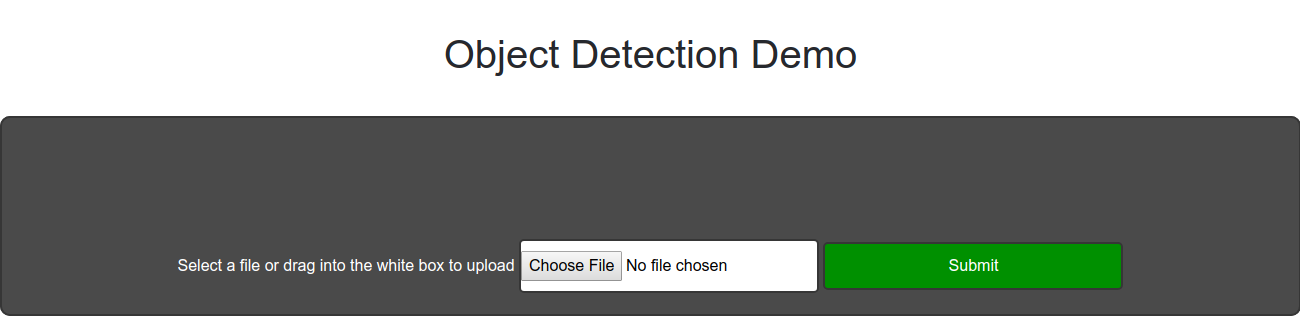
\includegraphics[width=15cm]{index}
	\caption{Simple Webpage to allow Image Upload}
	\label{fig:index}
\end{figure}

\section{Code Snippets}
\begin{flushleft}
Some interesting snippets of code from the application implementation have been provided below:
\end{flushleft}

\vspace{0.5cm}
\begin{figure}[ht!]
	\centering
	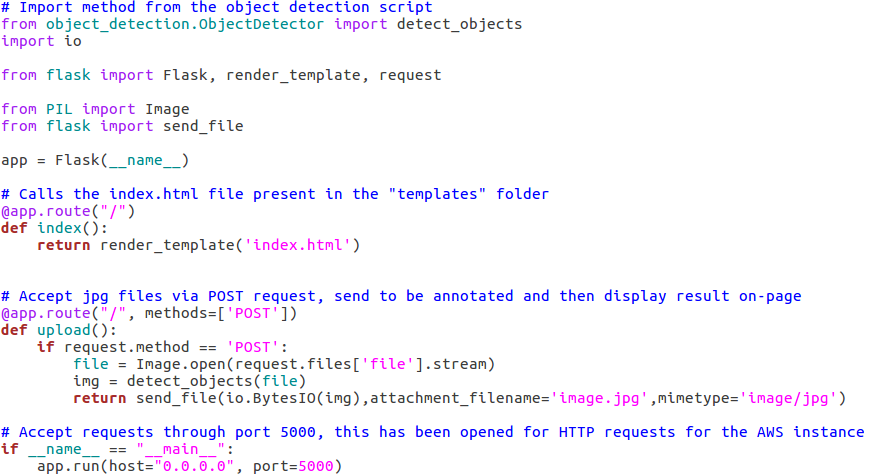
\includegraphics[width=15cm]{flask}
	\caption{Flask Application Code, calls Annotation Code}
	\label{fig:flask}
\end{figure}

\vspace{0.5cm}
\begin{figure}[ht!]
	\centering
	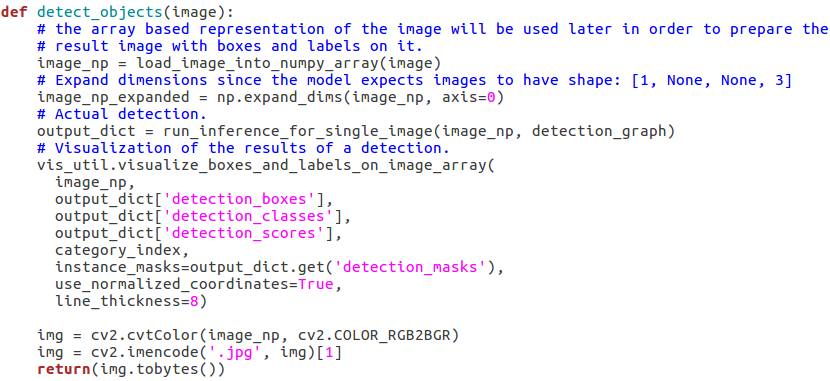
\includegraphics[width=15cm]{flask-2}
	\caption{Method called by Flask Application, accepts and returns image}
	\label{fig:flask-2}
\end{figure}

\newpage
\chapter{Final Conclusion and Discussion}
\section{Summary}
\begin{flushleft}
The primary purpose behind this project has been an investigation into how CNN's perform object detection and the issues encountered during this process. Once the research area for this project had been defined, a comprehsive literature review of the subject material was undertaken. One of the main objectives for the literature review was to develop and document an expansive knowledge of CNN's. A working knowledge of using tensorflow was also developed through a Udemy tutorial (\cite{udemy}). Once this knowledge had been gained, several experiments were undertaken in an attempt to replicate the results published in (\cite{yu2018bdd100k}). Although the full BDD100K dataset quickly proved far too complex to use in its entirety, a subsampled version of the dataset was sufficient for training instead. Although the results provided by Yu et al. were not replicated perfectly, results that were within an acceptable margin of error were obtained. Unfortunately financial constraints related to using AWS services did not allow for further experimentation, however I am satisfied with the results obtained throughout the experimentation phase of this project. Finally, a lightweight Flask application was built and deployed in order to allow users to interact with the models trained during the experimentation phase.
\end{flushleft}

\section{Future Work}
\begin{flushleft}
This project has very much served to foster a passion for the field of Computer Vision and object detection tasks specifically. This has been one of the very few projects for me where I have a genuine desire to continue work upon related projects after completion. I have several ideas as to how I am going to go about work upon future personal projects in this field.
\end{flushleft}

\subsection*{This Project}
\begin{flushleft}
With AWS costs forcing experimentation to stop for this project, there are several potential areas of future work that could be worth pursuing. With the Faster-RCNN Inception architecture producing good results albeit at the cost of annotation speed, I would like to investigate the possibility of using SSD or YOLO based Inception architectures, as I feel that this would help decrease annotation times and create a model more suited to performing accurate object detection in real-time. If I am to continue work on this project in future, opting for a more powerful AWS machine instance would also be a priority in order to aid detection in real-time. I would also like to investigate training a MobileNet architecture myself on the COCO dataset without image resizing, and then retrain this model using the BDD100K dataset. As mentioned above, the MobileNet architecture can produce similar results to other more complex architectures at a fraction of the computational costs (\cite{howard2017mobilenets}), so I feel that this solution could be a good trade off between performance and computation times.
\end{flushleft}

\subsection*{Future Projects}
\begin{flushleft}
One avenue that I am definitely going to be exploring is applying my experience gained from this project to my initial choice of project, a fish detector. With time constraints no longer an issue and a graduate salary allowing the purchase of camera equipment, I intend to begin the collation of a dataset for this project. Although the issue still remains of gaining the required domain knowledge to annotate species for training data, I am confident that with enough research I will be able to annotate some basic easily-identifiable species. Thus far, I have not been able to find any models that have been pretrained on a fish species dataset. I have however found some publically available datasets such as (\cite{fish}), which contains species of fish found in European waters, upon which it may be possible to train a model myself. I believe that then retraining this model using my collated dataset may potentially lead to positive results. This is going to be my primary personal project going forward.
\end{flushleft}

\printbibliography
\begin{appendices}
\chapter{Project Plan}
\begin{flushleft}
The following table outlines the delivery dates agreed upon with my supervisor for the sections of this report along with the implementation of the demo day product. Athough it was not followed strictly, it provides a general overview of how this project progressed over time.
\end{flushleft}

\begin{table}[ht!]
\begin{tabular}{|l|l|l|}
\hline
Chapter                   & Section                  & Est. Completion Date \\ \hline
Introduction              & Overview of Problem Area & 12/10/2018           \\ \hline
                          & Motivations              & 12/10/2018           \\ \hline
                          & Objectives               & 05/10/2018           \\ \hline
                          & Contribution             & 05/04/2019           \\ \hline
                          & Methodologies            & 05/04/2019           \\ \hline
                          & Project Plan             & 05/10/2018           \\ \hline
Background Research       & Intro to ML              & 19/10/2018           \\ \hline
                          & Intro to Neural Networks & 26/10/2018           \\ \hline
                          & Intro to CNN's           & 26/10/2018           \\ \hline
                          & Intro to Computer Vision & 03/11/2018           \\ \hline
                          & Tensorflow Tutorial      & 19/10/2018           \\ \hline          
Empirical Studies         & MobileNet Architecture   & 25/01/2019           \\ \hline
                          & Inception Architecture   & 25/02/2019           \\ \hline                   
Application Impl.         & Flask App                & 28/03/2019           \\ \hline
                          & Object Detector Script   & 28/03/2019           \\ \hline         
Final Conclusion          & Summary                  & 08/04/2019           \\ \hline
                          & Reflections              & 08/04/2019           \\ \hline
                          & Future Work              & 08/04/2019           \\ \hline                          
\end{tabular}
\caption{Delivery dates for project milestones}
\end{table}

\chapter{Poster}
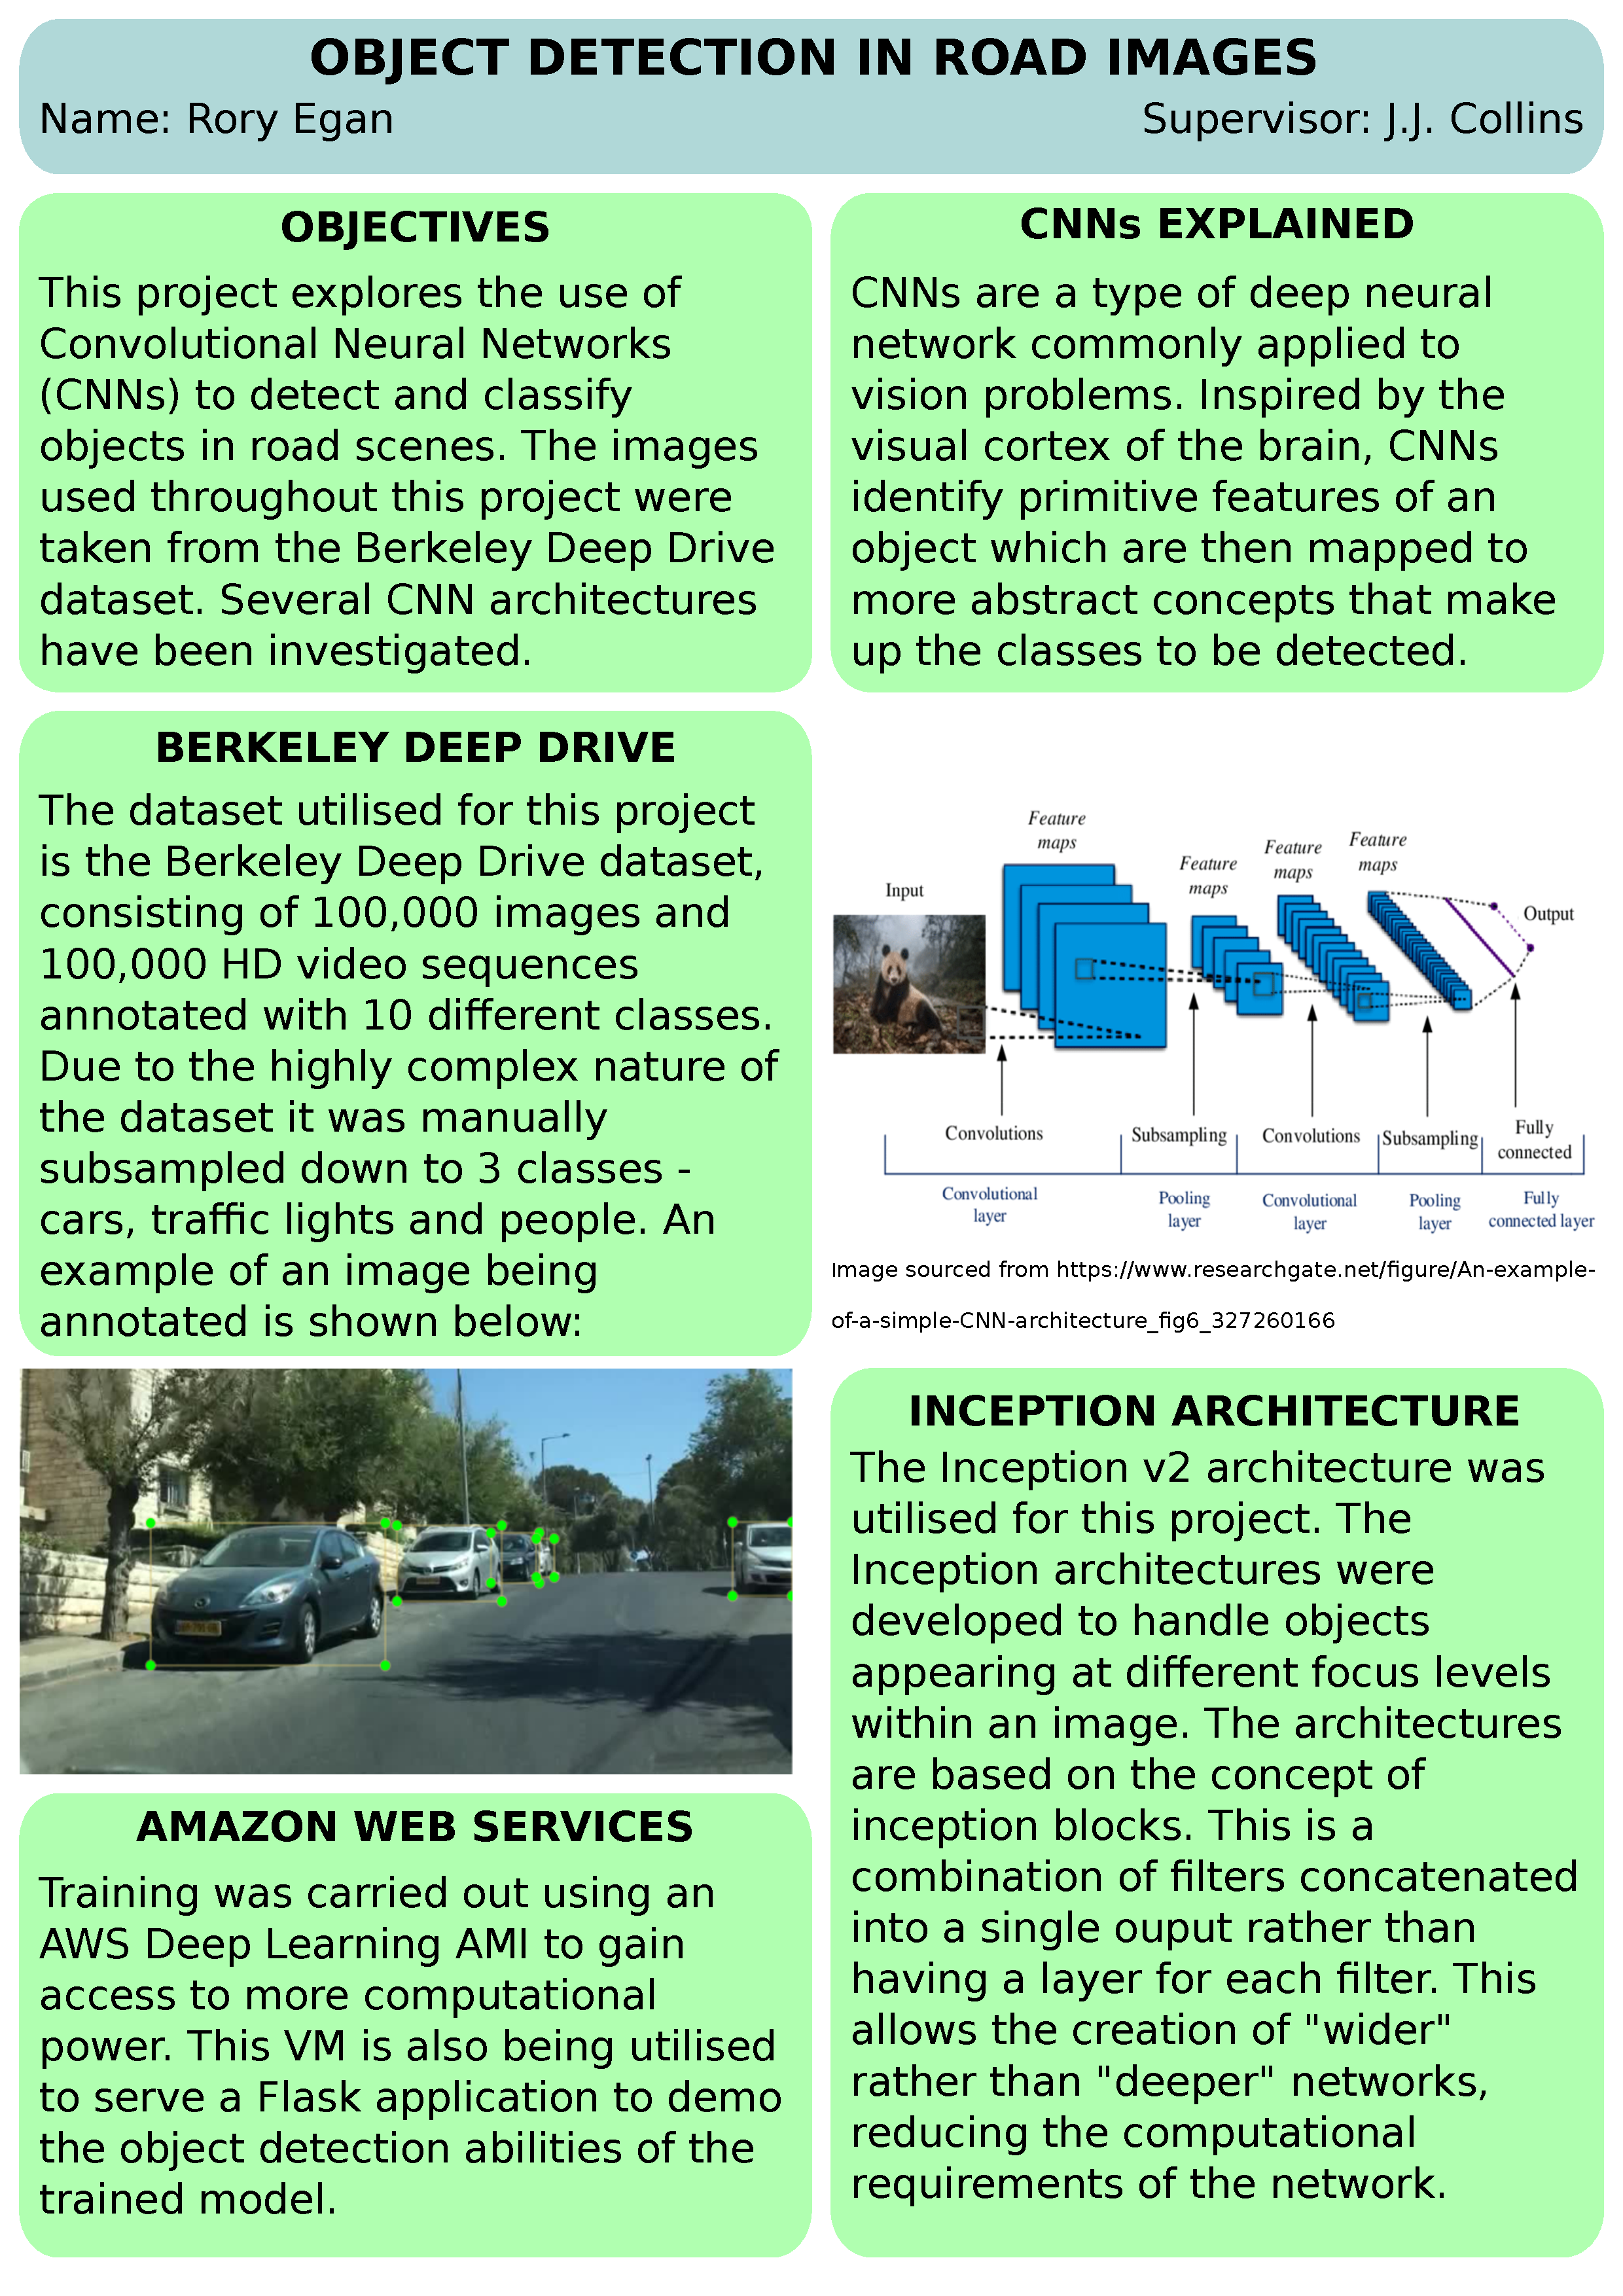
\includepdf{poster}
\end{appendices}
\end{document}